% ============================================
% chapter13_full_zh.tex — 第13章：域论
% 与第12章格式统一；正文、证明、例子与练习均保留
% ============================================

前面几部分发展了群、环和域这些基本代数结构的理论。接下来的两章研究域的性质，特别是那些由求解方程（例如简单方程 $x^2+1=0$）而产生的域，以及在进行“算术”（加、减、乘、除）时自然出现的域。优美的 Galois 理论把域的结构与某些相关群的结构联系起来，是基本的代数工具之一。它的应用包括尺规作图问题、有限域，以及 Abel 关于一般五次方程不可用根式求解的著名定理。

\chapter{域论}

\section{域扩张的基本理论}

回忆：域 $F$ 是一个带恒等元的交换环，并且其中每个非零元素都有逆。等价地，$F$ 的非零元素集合 $F^\times=F-\{0\}$ 在乘法下是一个阿贝尔群。

与任意域 $F$ 相联系的第一个不变量之一是它的特征，其定义如下：如果 $1_F$ 表示 $F$ 的恒等元，那么 $F$ 含有由 $1_F$ 生成的加法子群中的元素
\[
1_F,\quad 1_F+1_F,\quad 1_F+1_F+1_F,\ldots,
\]
这些元素未必全都不同。对正整数 $n$，令 $n\cdot 1_F=1_F+\cdots+1_F$（$n$ 次）。于是有两种可能：或者所有元素 $n\cdot 1_F$ 都互不相同，或者存在某个正整数 $n$ 使得 $n\cdot 1_F=0$。

\noindent\textbf{定义.} 域 $F$ 的\emph{特征}，记为 $\operatorname{ch}(F)$，定义为满足 $p\cdot 1_F=0$ 的最小正整数 $p$，如果这样的 $p$ 存在；若不存在这样的 $p$，则定义为 $0$。

容易看到
\[
n\cdot 1_F+m\cdot 1_F=(m+n)\cdot 1_F
\]
以及
\[
(n\cdot 1_F)(m\cdot 1_F)=mn\cdot 1_F \tag{13.1}
\]
对正整数 $m$ 和 $n$ 成立。由此可知，域的特征或者是 $0$，或者是一个素数 $p$（因此上面的定义中选用字母 $p$），因为若 $n=ab$ 是合数并且 $n\cdot 1_F=0$，则
\[
ab\cdot 1_F=(a\cdot 1_F)(b\cdot 1_F)=0,
\]
而由于 $F$ 是域，$a\cdot 1_F$ 或 $b\cdot 1_F$ 中有一个为 $0$，所以这样的最小整数必然是素数。还可推出，若 $n\cdot 1_F=0$，则 $n$ 被 $p$ 整除。

\noindent\textbf{命题 1.} 域 $F$ 的特征 $\operatorname{ch}(F)$ 或为 $0$，或为素数 $p$。若 $\operatorname{ch}(F)=p$，则对任意 $a\in F$，
\[
p\cdot a=\underbrace{a+a+\cdots+a}_{p\text{ 次}}=0.
\]

\begin{proof}
	只有第二个断言尚未证明；它立即来自 $F$ 中显然的等式
	\[
	p\cdot a=p\cdot(1_Fa)=(p\cdot 1_F)(a).
	\]
\end{proof}

\paragraph{注记：} 这种特征的概念也适用于任意整环，并且一个整环的特征与其分式域的特征相同。

\paragraph{例}
\begin{enumerate}[label=(\arabic*)]
	\item 域 $\mathbb Q$ 和 $\mathbb R$ 的特征都为 $0$：$\operatorname{ch}(\mathbb Q)=\operatorname{ch}(\mathbb R)=0$。整环 $\mathbb Z$ 的特征也为 $0$。
	\item 对任意素数 $p$，有限域 $\mathbb F_p=\mathbb Z/p\mathbb Z$ 的特征为 $p$。
	\item 系数在域 $\mathbb F_p$ 中的变量 $x$ 的多项式整环 $\mathbb F_p[x]$ 的特征为 $p$，它的分式域 $\mathbb F_p(x)$（系数在 $\mathbb F_p$ 中的关于 $x$ 的有理函数域）的特征也为 $p$。
\end{enumerate}

若对正整数 $n$ 定义 $(-n)\cdot 1_F=-(n\cdot 1_F)$，并定义 $0\cdot 1_F=0$，则由等式 (13.1) 得到一个自然环同态
\[
\varphi:\mathbb Z\longrightarrow F,
\qquad
n\longmapsto n\cdot 1_F,
\]
并且我们可通过注意到 $\ker(\varphi)=\operatorname{ch}(F)\mathbb Z$ 来解释 $F$ 的特征。对核取商给出 $\mathbb Z$ 或 $\mathbb Z/p\mathbb Z$ 到 $F$ 的一个嵌入（取决于 $\operatorname{ch}(F)=0$ 还是 $\operatorname{ch}(F)=p$）。由于 $F$ 是域，我们看到，取决于 $F$ 的特征，$F$ 含有一个同构于 $\mathbb Q$（$\mathbb Z$ 的分式域）或同构于 $\mathbb F_p=\mathbb Z/p\mathbb Z$（$\mathbb Z/p\mathbb Z$ 的分式域）的子域；并且在任一情形中，这个子域都是 $F$ 中含有 $1_F$ 的最小子域（即 $F$ 中由 $1_F$ 生成的域）。

\noindent\textbf{定义.} 域 $F$ 的\emph{素子域}是由 $F$ 的乘法恒等元 $1_F$ 生成的子域。它（同构于）$\mathbb Q$（若 $\operatorname{ch}(F)=0$）或 $\mathbb F_p$（若 $\operatorname{ch}(F)=p$）。

\paragraph{注记：} 我们通常把域 $F$ 的恒等元 $1_F$ 简记为 $1$。于是，在特征为 $p$ 的域中，有 $p\cdot 1=0$，这常常简写为 $p=0$（例如，在特征为 $2$ 的域中 $2=0$）。然而应当记住，这只是一个简写说法——元素“$p$”实际上是 $p\cdot 1_F$，并不是 $F$ 中一个不同的元素。鉴于命题 1 的第二个断言，这种记法是有用的。

\paragraph{例}
\begin{enumerate}[label=(\arabic*)]
	\item $\mathbb Q$ 和 $\mathbb R$ 的素子域都是 $\mathbb Q$。
	\item 域 $\mathbb F_p(x)$ 的素子域同构于 $\mathbb F_p$，由常数多项式给出。
\end{enumerate}

\noindent\textbf{定义.} 若 $K$ 是含有子域 $F$ 的域，则称 $K$ 是 $F$ 的\emph{扩域}（或简称为 $F$ 的\emph{扩张}），记为 $K/F$，也用图
\[
\begin{array}{c}
	K\\
	|\\
	F
\end{array}
\]
表示。特别地，每个域 $F$ 都是它的素子域的扩张。域 $F$ 有时称为该扩张的\emph{基域}。

域扩张的记号 $K/F$ 是“$K$ 在 $F$ 上”的简写，而不是 $K$ 对 $F$ 的商。

若 $K/F$ 是任意域扩张，则 $K$ 中定义的乘法使 $K$ 成为 $F$ 上的向量空间。特别地，每个域 $F$ 都可看作其素域上的向量空间。

\noindent\textbf{定义.} 域扩张 $K/F$ 的\emph{次数}（或\emph{相对次数}，或\emph{指数}），记为 $[K:F]$，是 $K$ 作为 $F$ 上向量空间的维数（即 $[K:F]=\dim_F K$）。若 $[K:F]$ 有限，则称该扩张为\emph{有限}的；否则称为\emph{无限}的。

一类重要的域扩张，是试图在给定域 $F$ 上求解方程而得到的扩张。例如，若 $F=\mathbb R$ 是实数域，那么简单方程 $x^2+1=0$ 在 $F$ 中没有解。于是产生一个问题：是否存在某个含有 $\mathbb R$ 的更大的域，使得这个方程在其中有解？正是这个问题促使 Gauss 引入了复数 $\mathbb C=\mathbb R+\mathbb R i$，其中 $i$ 被定义为满足 $i^2+1=0$。然后按照初等代数中熟悉的通常规则在 $\mathbb C$ 中定义加法和乘法，并检查这样定义的 $\mathbb C$ 事实上是一个域，即每个非零元素都有逆。

给定任意域 $F$ 和任意多项式 $p(x)\in F[x]$，可以提出类似问题：是否存在 $F$ 的扩张 $K$，含有方程 $p(x)=0$ 的一个解（即含有 $p(x)$ 的一个根）？注意，这里可假设多项式 $p(x)$ 在 $F[x]$ 中不可约，因为 $p(x)$ 的任意因子的一个根当然也是 $p(x)$ 的一个根。答案是肯定的，并且几乎立即来自我们关于多项式环 $F[x]$ 的工作。我们先回忆关于域同态的以下有用结果（第 7 章推论 10），它来自域 $F$ 的理想只有 $0$ 和 $F$ 这一事实。

\noindent\textbf{命题 2.} 设 $\varphi:F\longrightarrow F'$ 是域同态。则 $\varphi$ 或恒等于 $0$，或是单射；因此 $\varphi$ 的像或者是 $0$，或者同构于 $F$。

\noindent\textbf{定理 3.} 设 $F$ 是域，$p(x)\in F[x]$ 是不可约多项式。则存在一个含有 $F$ 的一个同构拷贝的域 $K$，使得 $p(x)$ 在 $K$ 中有根。把 $F$ 与这个同构拷贝等同起来，便说明存在 $F$ 的一个扩张，使得 $p(x)$ 有根。

\begin{proof}
	考虑多项式环 $F[x]$ 对由 $p(x)$ 生成的理想取商得到的商
	\[
	K=F[x]/(p(x)).
	\]
	由于假设 $p(x)$ 是 P.I.D. $F[x]$ 中的不可约多项式，理想 $(p(x))$ 是极大理想。因此 $K$ 实际上是一个域（这是第 7 章命题 12）。从 $F[x]$ 到商 $F[x]/(p(x))$ 的典范投影 $\pi$ 限制在 $F\subset F[x]$ 上，给出同态
	\[
	\varphi=\pi|_F:F\longrightarrow K,
	\]
	它并非恒等于 $0$，因为它把 $F$ 的恒等元 $1$ 映到 $K$ 的恒等元 $1$。因此由上面的命题，$\varphi(F)\cong F$ 是包含在 $K$ 中的 $F$ 的一个同构拷贝。我们把 $F$ 与它在 $K$ 中的同构像等同起来，并把 $F$ 看作 $K$ 的一个子域。若 $\bar{x}=\pi(x)$ 表示 $x$ 在商 $K$ 中的像，则
	\[
	\begin{aligned}
		p(\bar{x})&=\overline{p(x)} &&\text{（因为 }\pi\text{ 是同态）}\
		&=p(x)\pmod{p(x)} &&\text{在 }F[x]/(p(x))\text{ 中}\
		&=0 &&\text{在 }F[x]/(p(x))\text{ 中},
	\end{aligned}
	\]
	所以 $K$ 的确含有多项式 $p(x)$ 的一个根。因此 $K$ 是 $F$ 的一个扩张，且 $p(x)$ 在其中有根。
\end{proof}

稍后我们将使用这个结果来构造含有 $p(x)$ 的所有根的 $F$ 的扩张（这就是分裂域的概念，是 Galois 理论中一个核心的研究对象）。

为了更充分地理解上面构造的域 $K=F[x]/(p(x))$，给出这个域中元素的简单表示是有用的。由于 $F$ 是 $K$ 的子域，我们特别可以询问 $K$ 作为 $F$ 上向量空间的一组基。

\noindent\textbf{定理 4.} 设 $p(x)\in F[x]$ 是域 $F$ 上次数为 $n$ 的不可约多项式，设 $K$ 为域 $F[x]/(p(x))$。令
\[
\theta=x\bmod (p(x))\in K.
\]
则元素
\[
1,\theta,\theta^2,\ldots,\theta^{n-1}
\]
构成 $K$ 作为 $F$ 上向量空间的一组基，所以扩张次数为 $n$，即 $[K:F]=n$。因此
\[
K=\{a_0+a_1\theta+a_2\theta^2+\cdots+a_{n-1}\theta^{n-1}\mid a_0,a_1,\ldots,a_{n-1}\in F\}
\]
由所有 $\theta$ 的次数 $<n$ 的多项式组成。

\begin{proof}
	设 $a(x)\in F[x]$ 是任意系数在 $F$ 中的多项式。由于 $F[x]$ 是 Euclidean 整环（这是第 9 章定理 3），我们可以用 $p(x)$ 除 $a(x)$：
	\[
	a(x)=q(x)p(x)+r(x),\qquad q(x),r(x)\in F[x],\quad \deg r(x)<n.
	\]
	由于 $q(x)p(x)$ 属于理想 $(p(x))$，可知
	\[
	a(x)\equiv r(x)\pmod{p(x)},
	\]
	这说明 $F[x]/(p(x))$ 中的每个剩余类都由一个次数小于 $n$ 的多项式表示。因此，$1,x,x^2,\ldots,x^{n-1}$ 在商中的像 $1,\theta,\theta^2,\ldots,\theta^{n-1}$ 张成这个商作为 $F$ 上的向量空间。还需证明这些元素线性无关，从而形成商在 $F$ 上的一组基。
	
	如果 $K$ 中的元素 $1,\theta,\theta^2,\ldots,\theta^{n-1}$ 不是线性无关的，那么存在一个线性组合
	\[
	b_0+b_1\theta+b_2\theta^2+\cdots+b_{n-1}\theta^{n-1}=0
	\]
	在 $K$ 中成立，其中 $b_0,b_1,\ldots,b_{n-1}\in F$ 且不全为 $0$。这等价于
	\[
	b_0+b_1x+b_2x^2+\cdots+b_{n-1}x^{n-1}\equiv 0\pmod{p(x)},
	\]
	即
	\[
	p(x)\text{ 整除 } b_0+b_1x+b_2x^2+\cdots+b_{n-1}x^{n-1}
	\]
	在 $F[x]$ 中成立。但这是不可能的，因为 $p(x)$ 的次数为 $n$，而右边非零多项式的次数 $<n$。这证明 $1,\theta,\theta^2,\ldots,\theta^{n-1}$ 是 $K$ 在 $F$ 上的一组基，所以按照定义 $[K:F]=n$。定理最后的断言显然成立。
\end{proof}

这个定理给出了域 $F[x]/(p(x))$ 中元素的一种简单描述：它们是 $\theta$ 的次数 $<n$ 的多项式，其中 $\theta$ 是一个满足 $p(\theta)=0$ 的元素（在 $K$ 中）。剩下的只是说明如何对这种形式写出的元素作加法和乘法。商 $F[x]/(p(x))$ 中的加法就是通常的多项式加法。商 $F[x]/(p(x))$ 中多项式 $a(x)$ 与 $b(x)$ 的乘法，是先在 $F[x]$ 中求乘积 $a(x)b(x)$，再通过用 $p(x)$ 除 $a(x)b(x)$ 并求余式，找到陪集 $a(x)b(x)+(p(x))$ 的次数 $<n$ 的代表元（如上面的证明所示）。

这也可以容易地用 $\theta$ 来完成，如下：我们可以假设 $p(x)$ 是首一多项式（因为把它乘以一个常数不会改变它的根，也不会改变它生成的理想），设
\[
p(x)=x^n+p_{n-1}x^{n-1}+\cdots+p_1x+p_0.
\]
于是，在 $K$ 中，由于 $p(\theta)=0$，有
\[
\theta^n=-(p_{n-1}\theta^{n-1}+\cdots+p_1\theta+p_0),
\]
即 $\theta^n$ 是 $\theta$ 的较低次幂的线性组合。两边同乘以 $\theta$，并再用这些较低次幂替换右边出现的 $\theta^n$，可见 $\theta^{n+1}$ 也是 $\theta$ 的次数 $<n$ 的多项式。类似地，$\theta$ 的任意正幂都可以写成 $\theta$ 的次数 $<n$ 的多项式，因此 $\theta$ 的任意多项式都可以写成 $\theta$ 的次数 $<n$ 的多项式。现在，在 $K$ 中作乘法很容易：只要把两个次数 $<n$ 的 $\theta$ 多项式的乘积再写成另一个次数 $<n$ 的 $\theta$ 多项式。我们把这总结为：

\noindent\textbf{推论 5.} 设 $K$ 如定理 4 中所述，令 $a(\theta),b(\theta)\in K$ 为 $\theta$ 的两个次数 $<n$ 的多项式。则 $K$ 中的加法简单地定义为通常的多项式加法，而 $K$ 中的乘法定义为
\[
a(\theta)b(\theta)=r(\theta),
\]
其中 $r(x)$ 是在 $F[x]$ 中用 $p(x)$ 除多项式 $a(x)b(x)$ 后得到的余式（次数 $<n$）。

由上面已经证明的结果，这样在 $\theta$ 的次数 $<n$ 的多项式上定义的加法和乘法使 $K$ 成为一个域，所以也可以除以非零元素；这一点从运算定义本身看并不是立即显然的。

定理 4 中多项式 $p(x)$ 在 $F$ 上不可约这一点也很重要。一般来说，推论 5 中的加法和乘法（对任意多项式 $p(x)$ 都可用同样方式定义）若 $p(x)$ 不可约，并不会使 $\theta$ 的次数 $<n$ 的多项式构成一个域。事实上，一般情况下这个集合甚至不是整环（其结构由第 9 章命题 16 给出）。为了描述含有一般多项式 $f(x)$ 在 $F$ 上的一个根 $\theta$ 的域，需要把 $f(x)$ 在 $F[x]$ 中分解为不可约因子，然后对 $f(x)$ 的一个以 $\theta$ 为根的不可约因子 $p(x)$ 应用上面的结果。我们将在以下各节进一步考虑这一点。

\paragraph{例}
\begin{enumerate}[label=(\arabic*)]
	\item 若把这个构造应用到特殊情形 $F=\mathbb R$ 且 $p(x)=x^2+1$，则得到域
	\[
	\mathbb R[x]/(x^2+1),
	\]
	这是 $\mathbb R$ 的一个次数为 $2$ 的扩张，其中 $x^2+1$ 有一个根。这个域的元素形如 $a+b\theta$，其中 $a,b\in\mathbb R$。加法定义为
	\[
	(a+b\theta)+(c+d\theta)=(a+c)+(b+d)\theta. \tag{13.2a}
	\]
	作乘法时使用事实 $\theta^2+1=0$，即 $K$ 中 $\theta^2=-1$。（或者，注意到 $x^2$ 除以 $x^2+1$ 在 $\mathbb R[x]$ 中的余式也是 $-1$。）于是
	\begin{equation}
		\begin{aligned}
			(a+b\theta)(c+d\theta)&=ac+(ad+bc)\theta+bd\theta^2\\
			&=ac+(ad+bc)\theta+bd(-1)\\
			&=(ac-bd)+(ad+bc)\theta.
		\end{aligned}
		\tag{13.2b}
	\end{equation}
	这些公式，差别只在于把 $\theta$ 改写为 $i$，正是 $\mathbb C$ 中加法和乘法的公式。换句话说，映射
	\[
	\varphi:\mathbb R[x]/(x^2+1)\longrightarrow \mathbb C,
	\qquad
	a+bx\longmapsto a+bi
	\]
	是一个同态。由于它是双射（例如作为实数上的向量空间之间的映射），它是一个同构。注意，与其先假定 $\mathbb C$ 的存在（并伴随相当冗长地验证它事实上是一个域），我们本可以通过这个同构来定义 $\mathbb C$。于是它是一个域这一事实就是定理 4 的结果。
	
	\item 现在取 $F=\mathbb Q$ 为有理数域，并再次取 $p(x)=x^2+1$（当然，它仍在 $\mathbb Q$ 上不可约）。则同样的构造给出 $\mathbb Q$ 的一个次数为 $2$ 的域扩张 $\mathbb Q(i)$，它含有 $x^2+1$ 的一个根 $i$；加法和乘法公式与上面的 (13.2a) 和 (13.2b) 相同，只是现在 $a$ 与 $b$ 是 $\mathbb Q$ 的元素。
	
	\item 取 $F=\mathbb Q$ 且 $p(x)=x^2-2$，例如由 Eisenstein 判别法可知它在 $\mathbb Q$ 上不可约。于是我们得到 $\mathbb Q$ 的一个次数为 $2$ 的域扩张，它含有 $2$ 的一个平方根 $\theta$，记为 $\mathbb Q(\theta)$。若用 $\sqrt2$ 表示 $\theta$，则这个域的元素形如
	\[
	a+b\sqrt2,
	\qquad a,b\in\mathbb Q,
	\]
	加法定义为
	\[
	(a+b\sqrt2)+(c+d\sqrt2)=(a+c)+(b+d)\sqrt2,
	\]
	乘法定义为
	\[
	(a+b\sqrt2)(c+d\sqrt2)=(ac+2bd)+(ad+bc)\sqrt2.
	\]
	
	\item 令 $F=\mathbb Q$ 且 $p(x)=x^3-2$，它同样由 Eisenstein 判别法不可约。把 $p(x)$ 的一个根记为 $\theta$，我们得到域
	\[
	\mathbb Q[x]/(x^3-2)\cong\{a+b\theta+c\theta^2\mid a,b,c\in\mathbb Q\},
	\]
	其中 $\theta^3=2$，这是一个次数为 $3$ 的扩张。要在这个域中求例如 $1+\theta$ 的逆，可以如下进行：由 $\mathbb Q[x]$ 中的 Euclidean 算法，存在多项式 $a(x)$ 和 $b(x)$ 使得
	\[
	a(x)(1+x)+b(x)(x^3-2)=1
	\]
	（因为 $p(x)=x^3-2$ 不可约，它与每个次数较低的多项式都互素）。在商域中，这个方程说明 $a(\theta)$ 是 $1+\theta$ 的逆。在此情形下，一个简单计算表明可取 $a(x)=\frac13(x^2-x+1)$（且 $b(x)=-\frac13$），所以
	\[
	(1+\theta)^{-1}=\frac{\theta^2-\theta+1}{3}.
	\]
	
	\item 一般地，若 $\theta\in K$ 是不可约多项式
	\[
	p(x)=p_nx^n+p_{n-1}x^{n-1}+\cdots+p_1x+p_0
	\]
	的根，则可由
	\[
	\theta(p_n\theta^{n-1}+p_{n-1}\theta^{n-2}+\cdots+p_1)=-p_0
	\]
	计算 $\theta^{-1}\in K$，即
	\[
	\theta^{-1}=-\frac{1}{p_0}(p_n\theta^{n-1}+p_{n-1}\theta^{n-2}+\cdots+p_1)\in K
	\]
	（注意 $p_0\neq 0$，因为 $p(x)$ 不可约）。
	
	\paragraph{注记：} 在 $\mathbb C$ 的情形或例 (3) 中，这类扩张里逆的求法可能以“分母有理化”之名在初等代数中为人熟知。最后两个例子指出了一个比初等代数中临时性的做法更为一般的过程。
	
	\item 取 $F=\mathbb F_2$，即含有两个元素的有限域，并取 $p(x)=x^2+x+1$，我们先前已经检验过它在 $\mathbb F_2$ 上不可约。这里得到 $\mathbb F_2$ 的一个次数为 $2$ 的扩张
	\[
	\mathbb F_2[x]/(x^2+x+1)\cong\{a+b\theta\mid a,b\in\mathbb F_2\},
	\]
	其中 $\theta^2=-\theta-1=\theta+1$。这个域 $\mathbb F_2(\theta)$（含有四个元素）中的乘法定义为
	\[
	\begin{aligned}
		(a+b\theta)(c+d\theta)&=ac+(ad+bc)\theta+bd\theta^2\\
		&=ac+(ad+bc)\theta+bd(\theta+1)\\
		&=(ac+bd)+(ad+bc+bd)\theta.
	\end{aligned}
	\]
	
	\item 令 $F=k(t)$ 为域 $k$ 上变量 $t$ 的有理函数域（例如 $k=\mathbb Q$ 或 $k=\mathbb F_p$）。令 $p(x)=x^2-t\in F[x]$。则 $p(x)$ 不可约（它在 $k[t]$ 中关于素元 $(t)$ 是 Eisenstein 的）。若把一个根记为 $\theta$，则相应的次数为 $2$ 的域扩张 $F(\theta)$ 由元素
	\[
	\{a(t)+b(t)\theta\mid a(t),b(t)\in F\}
	\]
	组成，其中系数 $a(t)$ 与 $b(t)$ 是系数在 $k$ 中的 $t$ 的有理函数，并且 $\theta^2=t$。
\end{enumerate}

设 $F$ 是域 $K$ 的一个子域，且 $\alpha\in K$ 是 $K$ 的一个元素。那么 $K$ 中同时含有 $F$ 与 $\alpha$ 的子域组成的集合非空（例如 $K$ 本身就是这样的域）。由于子域的交仍是子域，于是存在唯一的含有 $F$ 与 $\alpha$ 的极小子域（即所有具有这个性质的子域的交）。若把 $\alpha$ 替换为 $K$ 中的一族元素 $\alpha,\beta,\ldots$，同样的说法也成立。

\noindent\textbf{定义.} 设 $K$ 是域 $F$ 的一个扩张，并令 $\alpha,\beta,\ldots\in K$ 是 $K$ 的一族元素。那么 $K$ 中同时含有 $F$ 和元素 $\alpha,\beta,
\ldots$ 的最小子域，记为 $F(\alpha,\beta,\ldots)$，称为由 $\alpha,\beta,\ldots$ 在 $F$ 上生成的域。

\noindent\textbf{定义.} 若域 $K$ 由单个元素 $\alpha$ 在 $F$ 上生成，即 $K=F(\alpha)$，则称 $K$ 是 $F$ 的\emph{单扩张}，元素 $\alpha$ 称为该扩张的\emph{本原元}。

稍后我们将刻画域 $F$ 的哪些扩张是单扩张。特别地，我们将证明，特征为 $0$ 的域的每个有限扩张都是单扩张。

当 $\alpha$ 是某个不可约多项式 $p(x)$ 的根时，由 $\alpha$ 在 $F$ 上生成的单扩张 $F(\alpha)$ 与定理 3 中构造的域之间的联系由下述定理给出：

\noindent\textbf{定理 6.} 设 $F$ 是域，$p(x)\in F[x]$ 是不可约多项式。设 $K$ 是 $F$ 的扩域，其中含有 $p(x)$ 的一个根 $\alpha$：$p(\alpha)=0$。令 $F(\alpha)$ 表示由 $\alpha$ 在 $F$ 上生成的 $K$ 的子域。则
\[
F(\alpha)\cong F[x]/(p(x)).
\]

\paragraph{注记：} 这个定理说的是，$F$ 上任意一个含有 $p(x)$ 的根的域，都含有一个同构于定理 3 中构造的 $F$ 的扩张的子域，并且这个域（在同构意义下）是含有这样一个根的 $F$ 的最小扩张。这个结果与定理 3 的区别在于，定理 6 假设某个域 $K$ 中存在 $p(x)$ 的根 $\alpha$，而定理 3 的要点则是证明确实存在这样的扩域 $K$。

\begin{proof}
	有一个自然同态
	\[
	\varphi:F[x]\longrightarrow F(\alpha)\subseteq K,
	\qquad
	a(x)\longmapsto a(\alpha),
	\]
	它通过把 $F$ 按恒等映射送到 $F$，把 $x$ 送到 $\alpha$，再扩张为环同态而得到（即关于 $x$ 的多项式 $a(x)$ 映到关于 $\alpha$ 的多项式 $a(\alpha)$）。由于假设 $p(\alpha)=0$，元素 $p(x)$ 属于 $\varphi$ 的核，所以得到一个诱导同态（仍记为 $\varphi$）
	\[
	\varphi:F[x]/(p(x))\longrightarrow F(\alpha).
	\]
	但由于 $p(x)$ 不可约，左边的商是一个域，并且 $\varphi$ 不是零映射（例如它在 $F$ 上是恒等映射），所以 $\varphi$ 是左边这个域到其像上的一个同构。因为这个像于是是 $F(\alpha)$ 的一个子域，且含有 $F$ 并含有 $\alpha$，由 $F(\alpha)$ 的定义，该映射必为满射，从而证明了定理。
\end{proof}

结合推论 5，当 $\alpha$ 是不可约多项式 $p(x)$ 的一个根时，这就确定了域 $F(\alpha)$：

\noindent\textbf{推论 7.} 若在定理 6 中 $p(x)$ 的次数为 $n$，则
\[
F(\alpha)=\{a_0+a_1\alpha+a_2\alpha^2+\cdots+a_{n-1}\alpha^{n-1}\mid a_0,a_1,\ldots,a_{n-1}\in F\}\subseteq K.
\]

描述由多于一个元素生成的域要更复杂；我们将在下一节回到这个问题。

\paragraph{例}
\begin{enumerate}[label=(\arabic*)]
	\item 在上面的例 (3) 中，我们已经确定了由元素 $\sqrt2\in\mathbb R$ 在 $\mathbb Q$ 上生成的域 $\mathbb Q(\sqrt2)$；我们富有暗示性地把方程 $x^2-2=0$ 的抽象解 $\theta$ 记为符号 $\sqrt2$，而这个符号在域 $\mathbb R$ 中有独立的含义（即 $2$ 的正平方根）。
	
	\item 方程 $x^2-2=0$ 在 $\mathbb R$ 中还有另一个解，即 $-\sqrt2$，$2$ 的负平方根。由这个解在 $\mathbb Q$ 上生成的域由元素
	\[
	\{a+b(-\sqrt2)\mid a,b\in\mathbb Q\}
	\]
	组成，并且它也同构于上面例 (3) 中的域（因而也同构于刚才考虑的域，其同构显式地由 $a+b\sqrt2\mapsto a-b\sqrt2$ 给出）。作为 $\mathbb R$ 的子集，它与例 (1) 中的元素集合相同。
	
	\item 类似地，若用符号 $\sqrt[3]{2}$ 表示 $\mathbb R$ 中 $2$ 的（正）立方根，则由 $\sqrt[3]{2}$ 在 $\mathbb Q$ 上于 $\mathbb R$ 中生成的域由元素
	\[
	\{a+b\sqrt[3]{2}+c(\sqrt[3]{2})^2\mid a,b,c\in\mathbb Q\}
	\]
	组成，并同构于上面例 (4) 中构造的域。
	
	\item 方程 $x^3-2=0$ 在 $\mathbb R$ 中没有更多解，但在 $\mathbb C$ 中有另外两个解，分别为
	\[
	\sqrt[3]{2}\left(\frac{-1+i\sqrt3}{2}\right)
	\quad\text{和}\quad
	\sqrt[3]{2}\left(\frac{-1-i\sqrt3}{2}\right)
	\]
	（这里 $\sqrt3$ 表示 $3$ 的正实平方根），这可以容易地检验。由这两个元素中的任意一个在 $\mathbb Q$ 上生成的域都是 $\mathbb C$ 的子域（但不是 $\mathbb R$ 的子域），并且二者都同构于前一例中构造的域（也同构于更早的例 (4)）。
\end{enumerate}

如定理 6 所表明的，不可约多项式 $p(x)$ 的根在代数上是不可区分的，其意义是，把不可约多项式的任意一个根添入而得到的域都是同构的。在上面最后两个例子中，把 $x^3-2=0$ 的三个可能的（复）根中任一个添入 $\mathbb Q$ 所得的域在代数上全都同构。这些域不是由它们的代数性质区分的，而是由它们的元素是否为实数来区分；这涉及连续运算。

同一个不可约多项式的不同根具有相同代数性质这一事实还可以稍作推广，如下：

令 $\varphi:F\to F'$ 是域同构。映射 $\varphi$ 诱导一个环同构（仍记为 $\varphi$）
\[
\varphi:F[x]\longrightarrow F'[x]
\]
它通过把 $\varphi$ 作用到 $F[x]$ 中多项式的系数上来定义。令 $p(x)\in F[x]$ 是不可约多项式，并令 $p'(x)\in F'[x]$ 是把映射 $\varphi$ 作用到 $p(x)$ 的系数上所得的多项式，即 $p(x)$ 在 $\varphi$ 下的像。同构 $\varphi$ 把极大理想 $(p(x))$ 映到理想 $(p'(x))$，所以这个理想也极大，从而说明 $p'(x)$ 在 $F'[x]$ 中也不可约。下述定理说明，把 $p(x)$ 的一个根添入 $F$ 所得的域，与把 $p'(x)$ 的一个根添入 $F'$ 所得的域具有相同的代数结构（即同构）：

\noindent\textbf{定理 8.} 设 $\varphi:F\to F'$ 是域同构。设 $p(x)\in F[x]$ 是不可约多项式，$p'(x)\in F'[x]$ 是把映射 $\varphi$ 作用到 $p(x)$ 的系数上所得的不可约多项式。令 $\alpha$ 为 $p(x)$ 的一个根（在 $F$ 的某个扩张中），令 $\beta$ 为 $p'(x)$ 的一个根（在 $F'$ 的某个扩张中）。则存在同构
\[
\sigma:F(\alpha)\longrightarrow F'(\beta),
\qquad
\alpha\longmapsto \beta,
\]
它把 $\alpha$ 映到 $\beta$ 并延拓 $\varphi$，即其限制在 $F$ 上等于同构 $\varphi$。

\begin{proof}
	如上所述，同构 $\varphi$ 诱导从 $F[x]$ 到 $F'[x]$ 的一个自然同构，它把极大理想 $(p(x))$ 映到极大理想 $(p'(x))$。对这些理想取商，得到域同构
	\[
	F[x]/(p(x))\cong F'[x]/(p'(x)).
	\]
	由定理 6，左边的域同构于 $F(\alpha)$；同样由该定理，右边的域同构于 $F'(\beta)$。复合这些同构，得到同构 $\sigma$。显然这个同构限制到 $F$ 上就是 $\varphi$，证明完成。
\end{proof}

这个延拓定理在我们稍后考虑 Galois 理论时将相当有用。它可由图
\[
\begin{array}{ccc}
	\sigma:
	F(\alpha)&\longrightarrow&F'(\beta)\\
	&\alpha\longmapsto\beta&\\[-2pt]
	\varphi:\quad F&\longrightarrow&F'
\end{array}
\]
表示。

\subsection*{练习}
\begin{enumerate}[label=\arabic*.]
	\item 证明 $p(x)=x^3+9x+6$ 在 $\mathbb Q[x]$ 中不可约。令 $\theta$ 为 $p(x)$ 的一个根。求 $\mathbb Q(\theta)$ 中 $1+\theta$ 的逆。
	
	\item 证明 $x^3-2x-2$ 在 $\mathbb Q$ 上不可约，并令 $\theta$ 为其一个根。在 $\mathbb Q(\theta)$ 中计算
	\[
	(1+\theta)(1+\theta+\theta^2)
	\quad\text{和}\quad
	\frac{1+\theta}{1+\theta+\theta^2}.
	\]
	
	\item 证明 $x^3+x+1$ 在 $\mathbb F_2$ 上不可约，并令 $\theta$ 为其一个根。计算 $\mathbb F_2(\theta)$ 中 $\theta$ 的各次幂。
	
	\item 直接证明映射
	\[
	a+b\sqrt2\longmapsto a-b\sqrt2
	\]
	是 $\mathbb Q(\sqrt2)$ 到自身的一个同构。
	
	\item 设 $\alpha$ 是 $\mathbb Z[x]$ 中某个首一多项式的有理根。证明 $\alpha$ 是整数。
	
	\item 证明：若 $\alpha$ 是
	\[
	a_nx^n+a_{n-1}x^{n-1}+\cdots+a_1x+a_0
	\]
	的一个根，则 $a_n\alpha$ 是下列首一多项式的一个根：
	\[
	x^n+a_{n-1}x^{n-1}+a_na_{n-2}x^{n-2}+\cdots+a_n^{n-2}a_1x+a_n^{n-1}a_0.
	\]
	
	\item 证明当 $n\neq -1,3,5$ 时，$x^3-nx+2$ 不可约。
	
	\item 证明 $x^5-ax-1\in\mathbb Z[x]$ 不可约，除非 $a=0,2$ 或 $-1$。前两个值对应线性因子，第三个值对应分解
	\[
	(x^2-x+1)(x^3+x^2-1).
	\]
\end{enumerate}
\section{代数扩张}

设 $F$ 是一个域，设 $K$ 是 $F$ 的一个扩张。

\noindent\textbf{定义.} 元素 $\alpha\in K$ 称为在 $F$ 上是\emph{代数的}，如果 $\alpha$ 是某个非零多项式 $f(x)\in F[x]$ 的根。如果 $\alpha$ 在 $F$ 上不是代数的（即，它不是任意一个系数在 $F$ 中的非零多项式的根），则称 $\alpha$ 在 $F$ 上是\emph{超越的}。扩张 $K/F$ 称为\emph{代数扩张}，如果 $K$ 的每个元素都在 $F$ 上是代数的。

注意，如果 $\alpha$ 在域 $F$ 上是代数的，那么它也在 $F$ 的任意扩域 $L$ 上是代数的（若以 $\alpha$ 为根的 $f(x)$ 的系数在 $F$ 中，则这些系数也在 $L$ 中）。

\noindent\textbf{命题 9.} 设 $\alpha$ 在 $F$ 上是代数的。则存在唯一的首一不可约多项式
\[
m_{\alpha,F}(x)\in F[x]
\]
以 $\alpha$ 为根。一个多项式 $f(x)\in F[x]$ 以 $\alpha$ 为根，当且仅当 $m_{\alpha,F}(x)$ 在 $F[x]$ 中整除 $f(x)$。

\begin{proof}
	设 $g(x)\in F[x]$ 是所有以 $\alpha$ 为根的多项式中次数最小的一个。把 $g(x)$ 乘以一个常数，我们可以假设 $g(x)$ 是首一的。若 $g(x)$ 在 $F[x]$ 中可约，例如
	\[
	g(x)=a(x)b(x),
	\]
	其中 $a(x),b(x)\in F[x]$ 的次数都小于 $g(x)$ 的次数，则在 $K$ 中有
	\[
	g(\alpha)=a(\alpha)b(\alpha).
	\]
	由于 $K$ 是域，或者 $a(\alpha)=0$，或者 $b(\alpha)=0$，这与 $g(x)$ 的次数的最小性矛盾。因此 $g(x)$ 是一个以 $\alpha$ 为根的首一不可约多项式。
	
	现在设 $f(x)\in F[x]$ 是任意一个以 $\alpha$ 为根的多项式。由 $F[x]$ 中的 Euclidean 算法，存在多项式 $q(x),r(x)\in F[x]$ 使得
	\[
	f(x)=q(x)g(x)+r(x),\qquad \deg r(x)<\deg g(x).
	\]
	于是，在 $K$ 中
	\[
	f(\alpha)=q(\alpha)g(\alpha)+r(\alpha).
	\]
	由于 $\alpha$ 同时是 $f(x)$ 和 $g(x)$ 的根，得到 $r(\alpha)=0$；除非 $r(x)=0$，这将与 $g(x)$ 的次数最小性矛盾。因此 $g(x)$ 整除 $F[x]$ 中任意以 $\alpha$ 为根的多项式 $f(x)$；特别地，它将整除任意另一个以 $\alpha$ 为根的首一不可约多项式。这证明了 $m_{\alpha,F}(x)=g(x)$ 的唯一性，并完成命题的证明。
\end{proof}

\noindent\textbf{推论 10.} 若 $L/F$ 是域扩张，并且 $\alpha$ 同时在 $F$ 和 $L$ 上是代数的，则 $m_{\alpha,L}(x)$ 在 $L[x]$ 中整除 $m_{\alpha,F}(x)$。

\begin{proof}
	这立即来自把命题 9 的第二个断言应用于 $L$，因为 $m_{\alpha,F}(x)$ 是 $L[x]$ 中以 $\alpha$ 为根的多项式。
\end{proof}

\noindent\textbf{定义.} 命题 9 中的多项式 $m_{\alpha,F}(x)$（如果域 $F$ 已由上下文明确，也简记为 $m_\alpha(x)$）称为 $\alpha$ 在 $F$ 上的\emph{极小多项式}。$m_\alpha(x)$ 的次数称为 $\alpha$ 的\emph{次数}。

注意，由命题可知，$F$ 上一个以 $\alpha$ 为根的首一多项式是 $\alpha$ 在 $F$ 上的极小多项式，当且仅当它在 $F$ 上不可约。练习 20 给出了计算 $\alpha$ 在 $F$ 上的极小多项式的一种方法；而 Gröbner 基理论可以用来计算 $F(\alpha)$ 中其他元素的极小多项式（参见第 15.1 节命题 10 与练习 48）。

\noindent\textbf{命题 11.} 设 $\alpha$ 在域 $F$ 上是代数的，设 $F(\alpha)$ 是由 $\alpha$ 在 $F$ 上生成的域。则
\[
F(\alpha)\cong F[x]/(m_\alpha(x)),
\]
因而特别地
\[
[F(\alpha):F]=\deg m_\alpha(x)=\deg \alpha,
\]
也就是说，$\alpha$ 在 $F$ 上的次数就是它生成的扩张的次数。

\begin{proof}
	这立即来自定理 6。
\end{proof}

\paragraph{例}
\begin{enumerate}[label=(\arabic*)]
	\item $\sqrt2$ 在 $\mathbb Q$ 上的极小多项式是 $x^2-2$，并且 $\sqrt2$ 在 $\mathbb Q$ 上的次数为 $2$：
	\[
	[\mathbb Q(\sqrt2):\mathbb Q]=2.
	\]
	\item $\sqrt[3]{2}$ 在 $\mathbb Q$ 上的极小多项式是 $x^3-2$，并且 $\sqrt[3]{2}$ 在 $\mathbb Q$ 上的次数为 $3$：
	\[
	[\mathbb Q(\sqrt[3]{2}):\mathbb Q]=3.
	\]
	\item 类似地，对任意 $n>1$，多项式 $x^n-2$ 在 $\mathbb Q$ 上不可约，因为它满足 Eisenstein 判别法。把这个多项式的一个根记为 $\sqrt[n]{2}$（照常，若我们想把这个根看作 $\mathbb R$ 中的元素，就保留这个符号表示 $2$ 的正 $n$ 次根；而一般地，这个符号表示代数上不可区分的抽象解中的任意一个），则
	\[
	[\mathbb Q(\sqrt[n]{2}):\mathbb Q]=n.
	\]
	\item 一个元素 $\alpha$ 的极小多项式和次数依赖于基域。例如，在 $\mathbb R$ 上，元素 $\sqrt[n]{2}$ 的次数为 $1$，其极小多项式为
	\[
	m_{\alpha,\mathbb R}(x)=x-\sqrt[n]{2}.
	\]
	\item 考虑 $\mathbb Q$ 上的多项式
	\[
	p(x)=x^3-3x-1,
	\]
	它在 $\mathbb Q$ 上不可约，因为它是一个没有有理根的三次多项式（参见第 9 章命题 11）。因此，对 $p(x)$ 的任意根 $\alpha$，都有 $[\mathbb Q(\alpha):\mathbb Q]=3$。为了以后引用，我们注意到，在实数上快速画出这个函数的图像可见，该图像在区间 $[0,2]$ 中恰好与 $x$ 轴相交一次；也就是说，恰有一个实数 $\alpha$，$0<\alpha<2$，满足
	\[
	\alpha^3-3\alpha-1=0.
	\]
\end{enumerate}

\noindent\textbf{命题 12.} 元素 $\alpha$ 在 $F$ 上是代数的，当且仅当单扩张 $F(\alpha)/F$ 是有限的。更精确地，若 $\alpha$ 是 $F$ 上一个次数为 $n$ 的扩张中的元素，则 $\alpha$ 满足一个在 $F$ 上次数至多为 $n$ 的多项式；而若 $\alpha$ 满足一个在 $F$ 上次数为 $n$ 的多项式，则 $F(\alpha)$ 在 $F$ 上的次数至多为 $n$。

\begin{proof}
	若 $\alpha$ 在 $F$ 上是代数的，则扩张 $F(\alpha)/F$ 的次数就是 $\alpha$ 在 $F$ 上的极小多项式的次数。因此该扩张是有限的；若 $\alpha$ 满足一个次数为 $n$ 的多项式，则该扩张次数至多为 $n$。反过来，假设 $\alpha$ 是 $F$ 上次数为 $n$ 的一个扩张中的元素（例如，若 $[F(\alpha):F]=n$）。那么 $F(\alpha)$ 中的 $n+1$ 个元素
	\[
	1,\alpha,\alpha^2,
	\ldots,\alpha^n
	\]
	在 $F$ 上线性相关，也就是说，存在不全为 $0$ 的 $b_0,b_1,b_2,\ldots,b_n\in F$，使得
	\[
	b_0+b_1\alpha+b_2\alpha^2+\cdots+b_n\alpha^n=0.
	\]
	因此 $\alpha$ 是一个系数在 $F$ 中的非零多项式（次数 $\leq n$）的根，这证明 $\alpha$ 在 $F$ 上是代数的，也证明了命题的第二个断言。
\end{proof}

\noindent\textbf{推论 13.} 若扩张 $K/F$ 是有限的，则它是代数扩张。

\begin{proof}
	若 $\alpha\in K$，则子域 $F(\alpha)$ 特别是 $K$ 作为 $F$ 上向量空间的一个子空间。因此 $[F(\alpha):F]\leq [K:F]$，所以由命题可知 $\alpha$ 在 $F$ 上是代数的。
\end{proof}

\paragraph{注记：} 下面我们将证明这个结果的某种逆命题（定理 17），但注意到存在无限的代数扩张（稍后我们将看到一个例子），所以这个推论的字面逆命题不为真。

\paragraph{例：（特征不为 $2$ 的域的二次扩张）}
设 $F$ 是一个特征不为 $2$ 的域（例如，任意特征为 $0$ 的域，如 $\mathbb Q$），设 $K$ 是 $F$ 的一个次数为 $2$ 的扩张，$[K:F]=2$。令 $\alpha$ 为 $K$ 中任意一个不属于 $F$ 的元素。由上面的命题，$\alpha$ 满足一个在 $F$ 上次数至多为 $2$ 的方程。这个方程不可能次数为 $1$，因为按假设 $\alpha$ 不是 $F$ 的元素。因此 $\alpha$ 的极小多项式是一个首一二次多项式
\[
m_\alpha(x)=x^2+bx+c,\qquad b,c\in F.
\]
由于 $F\subset F(\alpha)\subset K$，并且 $F(\alpha)$ 作为 $F$ 上向量空间已经是 $2$ 维的，我们有
\[
K=F(\alpha).
\]

这个二次方程的根可以由二次公式确定；该公式在任意特征不为 $2$ 的域上都是有效的（这个公式像初等代数中一样由配方得到）：
\[
\alpha=\frac{-b\pm\sqrt{b^2-4c}}{2}
\]
（要求 $F$ 的特征不为 $2$ 的原因是我们必须除以 $2$）。这里 $b^2-4c$ 在 $F$ 中不是平方，因为 $\alpha$ 不是 $F$ 的元素；符号 $\sqrt{b^2-4c}$ 表示 $K$ 中方程
\[
x^2-(b^2-4c)=0
\]
的一个根（见下一段末尾）。注意，在这里并没有一个类似于在 $\mathbb R$ 中选取 $2$ 的正平方根的自然选择；这些根在代数上是不可区分的。

现在 $F(\alpha)=F(\sqrt{b^2-4c})$，理由如下：由上面的公式，$\alpha$ 是右边这个域的元素，所以
\[
F(\alpha)\subset F(\sqrt{b^2-4c}).
\]
反过来，
\[
\sqrt{b^2-4c}=\pm(b+2\alpha)
\]
说明 $\sqrt{b^2-4c}$ 是 $F(\alpha)$ 的元素，于是得到反向包含
\[
F(\sqrt{b^2-4c})\subset F(\alpha),
\]
并且顺便说明方程 $x^2-(b^2-4c)=0$ 在 $K$ 中确实有一个解。

由此可知，$F$ 的任意次数为 $2$ 的扩张 $K$ 都具有形式 $F(\sqrt D)$，其中 $D$ 是 $F$ 中一个不是平方的元素；反过来，每个这样的扩张都是 $F$ 的次数为 $2$ 的扩张。因此，域 $F$ 的次数为 $2$ 的扩张称为 $F$ 的\emph{二次扩张}。

假设 $F$ 是域 $K$ 的子域，而 $K$ 又是域 $L$ 的子域。于是有三个相关的扩张次数——$K$ 和 $L$ 作为 $F$ 上向量空间的维数，以及 $L$ 作为 $K$ 上向量空间的维数。

\noindent\textbf{定理 14.} 设 $F\subset K\subset L$ 是域。则
\[
[L:F]=[L:K][K:F],
\]
也就是说，扩张次数是可乘的；其中，如果等式一边为无限，则另一边也为无限。用图表示为
\[
\begin{array}{ccccc}
	& & [L:F] & & \\
	F & \subset & K & \subset & L\\
	\underbrace{\hspace{2.0cm}}_{[K:F]} & & & \underbrace{\hspace{2.0cm}}_{[L:K]}
\end{array}
\]

\begin{proof}
	首先假设 $[L:K]=m$ 且 $[K:F]=n$ 都有限。令 $\alpha_1,\alpha_2,\ldots,\alpha_m$ 是 $L$ 在 $K$ 上的一组基，令 $\beta_1,\beta_2,\ldots,\beta_n$ 是 $K$ 在 $F$ 上的一组基。那么 $L$ 的每个元素都可写成线性组合
	\[
	a_1\alpha_1+a_2\alpha_2+\cdots+a_m\alpha_m,
	\]
	其中 $a_1,\ldots,a_m$ 是 $K$ 的元素，因此又是 $\beta_1,\ldots,\beta_n$ 的 $F$-线性组合：
	\[
	a_i=b_{i1}\beta_1+b_{i2}\beta_2+\cdots+b_{in}\beta_n,
	\qquad i=1,2,
	\ldots,m, \tag{13.3}
	\]
	其中 $b_{ij}$ 是 $F$ 的元素。把这些表达式代入上面 $a_i$ 的位置可见，$L$ 的每个元素都可写成
	\[
	\sum_{\substack{i=1,2,\ldots,m\\ j=1,2,\ldots,n}} b_{ij}\alpha_i\beta_j
	\]
	的线性组合，系数在 $F$ 中。因此这 $mn$ 个元素 $\alpha_i\beta_j$ 张成 $L$ 作为 $F$ 上的向量空间。
	
	现在假设在 $L$ 中有一个线性关系
	\[
	\sum_{\substack{i=1,2,\ldots,m\\ j=1,2,\ldots,n}} b_{ij}\alpha_i\beta_j=0,
	\]
	其中 $b_{ij}$ 在 $F$ 中。按上面的公式 (13.3) 定义元素 $a_i\in K$，则这个线性关系可写成
	\[
	a_1\alpha_1+a_2\alpha_2+\cdots+a_m\alpha_m=0.
	\]
	由于 $\alpha_i$ 是 $L$ 在 $K$ 上的一组基，所有系数 $a_i$，$i=1,2,\ldots,m$，都必须为 $0$；也就是说，
	\[
	b_{i1}\beta_1+b_{i2}\beta_2+\cdots+b_{in}\beta_n=0,
	\qquad i=1,2,\ldots,m,
	\]
	是在 $K$ 中的等式。由于现在 $\beta_j$，$j=1,2,\ldots,n$，构成 $K$ 在 $F$ 上的一组基，这推出所有 $i,j$ 都有 $b_{ij}=0$。因此元素 $\alpha_i\beta_j$ 在 $F$ 上线性无关，所以形成 $L$ 在 $F$ 上的一组基，并且
	\[
	[L:F]=mn=[L:K][K:F],
	\]
	如所要证明。
	
	若 $[K:F]$ 为无限，则 $K$ 中有无限多个在 $F$ 上线性无关的元素，因而 $L$ 中也有这些元素，所以 $[L:F]$ 也是无限的。类似地，若 $[L:K]$ 为无限，则 $L$ 中有无限多个在 $K$ 上线性无关的元素，当然也在 $F$ 上线性无关，所以 $[L:F]$ 仍为无限。最后，若 $[L:K]$ 和 $[K:F]$ 都有限，则上面的证明说明 $[L:F]$ 有限；因此 $[L:F]$ 为无限意味着 $[L:K]$ 与 $[K:F]$ 中至少有一个为无限。证明完成。
\end{proof}

\paragraph{注记：} 注意这个结果与第一部分中关于群的阶的结果相似。与涉及群的图表一样，我们将经常在域图中标出扩张的相对次数。

扩张次数的可乘性在计算中极为有用。一个特别的应用如下：

\noindent\textbf{推论 15.} 设 $L/F$ 是有限扩张，设 $K$ 是 $L$ 的任意含有 $F$ 的子域，$F\subset K\subset L$。则 $[K:F]$ 整除 $[L:F]$。

\begin{proof}
	这是立即的。
\end{proof}

\paragraph{例}
\begin{enumerate}[label=(\arabic*)]
	\item 元素 $\sqrt2$ 不属于域 $\mathbb Q(\alpha)$，其中 $\alpha$ 是 $x^3-3x-1$ 在 $0$ 与 $2$ 之间的实根；因为我们已经确定
	\[
	[\mathbb Q(\sqrt2):\mathbb Q]=2,
	\qquad [\mathbb Q(\alpha):\mathbb Q]=3,
	\]
	而 $2$ 不整除 $3$。注意，直接证明 $\sqrt2$ 不能写成 $1,\alpha,\alpha^2$ 的有理线性组合并不那么容易。
	\item 照常令 $\sqrt[6]{2}$ 表示 $2$ 的正实六次根。则
	\[
	[\mathbb Q(\sqrt[6]{2}):\mathbb Q]=6.
	\]
	由于 $(\sqrt[6]{2})^3=\sqrt2$，我们有
	\[
	\mathbb Q(\sqrt2)\subset \mathbb Q(\sqrt[6]{2}),
	\]
	并且由扩张次数的可乘性，
	\[
	[\mathbb Q(\sqrt[6]{2}):\mathbb Q(\sqrt2)]=3.
	\]
	这给出域图
	\[
	\begin{array}{ccccc}
		\mathbb Q & \subset & \mathbb Q(\sqrt2) & \subset & \mathbb Q(\sqrt[6]{2})\\
		& 2 & & 3 & \\
		\multicolumn{5}{c}{[\mathbb Q(\sqrt[6]{2}):\mathbb Q]=6.}
	\end{array}
	\]
	特别地，这说明 $\sqrt[6]{2}$ 在 $\mathbb Q(\sqrt2)$ 上的极小多项式次数为 $3$。因此它就是多项式
	\[
	x^3-\sqrt2.
	\]
	注意，直接说明这个多项式在 $\mathbb Q(\sqrt2)$ 上不可约并非完全平凡。
\end{enumerate}

由定理 14，有限扩张的有限扩张仍为有限。接下来的结果使用这一点来说明，由有限多个代数元素生成的扩张是有限的（推广命题 12）。

\noindent\textbf{定义.} 扩张 $K/F$ 称为\emph{有限生成的}，如果存在 $K$ 中的元素 $\alpha_1,\alpha_2,\ldots,\alpha_k$，使得
\[
K=F(\alpha_1,\alpha_2,\ldots,\alpha_k).
\]

回忆：在域 $K$ 中由一组元素在 $F$ 上生成的域，是 $K$ 中含有这些元素和 $F$ 的最小子域。下一个引理将说明，对于有限生成扩张，这个域可以通过一系列单扩张递归地得到。

\noindent\textbf{引理 16.} $F(\alpha,\beta)=(F(\alpha))(\beta)$，即，由 $\alpha$ 和 $\beta$ 在 $F$ 上生成的域，就是由 $\beta$ 在 $\alpha$ 生成的域 $F(\alpha)$ 上生成的域。

\begin{proof}
	这来自所讨论的域的最小性。域 $F(\alpha,\beta)$ 含有 $F$ 和 $\alpha$，因此含有域 $F(\alpha)$；又由于它也含有 $\beta$，由域 $(F(\alpha))(\beta)$ 的最小性得到包含
	\[
	(F(\alpha))(\beta)\subset F(\alpha,\beta).
	\]
	由于域 $(F(\alpha))(\beta)$ 含有 $F$、$\alpha$ 和 $\beta$，由 $F(\alpha,\beta)$ 的最小性得到反向包含
	\[
	F(\alpha,\beta)\subset (F(\alpha))(\beta),
	\]
	这证明了引理。
\end{proof}

由引理，我们有
\[
K=F(\alpha_1,\alpha_2,\ldots,\alpha_k)
=(F(\alpha_1,\alpha_2,\ldots,\alpha_{k-1}))(\alpha_k),
\]
于是通过迭代可见，$K$ 是这样得到的：先取由 $\alpha_1$ 在 $F$ 上生成的域 $F_1$，然后取由 $\alpha_2$ 在 $F_1$ 上生成的域 $F_2$（这一点很重要），依次进行，直到 $F_k=K$。这给出一列域：
\[
F=F_0\subset F_1\subset F_2\subset \cdots\subset F_k=K,
\]
其中
\[
F_{i+1}=F_i(\alpha_{i+1}),\qquad i=0,1,\ldots,k-1.
\]

现在假设元素 $\alpha_1,\alpha_2,\ldots,\alpha_k$ 在 $F$ 上都是代数的，次数分别为 $n_1,n_2,\ldots,n_k$（于是先验地它们在 $F$ 的任意扩域上也都是代数的）。那么这列扩张是命题 11 中所考虑的那种单扩张。相对扩张次数 $[F_{i+1}:F_i]$ 等于 $\alpha_{i+1}$ 在 $F_i$ 上的极小多项式次数，该次数至多为 $n_{i+1}$（并且当且仅当 $\alpha_{i+1}$ 在 $F$ 上的极小多项式在 $F_i$ 上仍不可约时，等于 $n_{i+1}$）。由扩张次数的可乘性，我们看到
\[
[K:F]=[F_k:F_{k-1}][F_{k-1}:F_{k-2}]\cdots [F_1:F_0]
\]
也是有限的，并且 $\leq n_1n_2\cdots n_k$。

这也给出了 $F(\alpha_1,\alpha_2,\ldots,\alpha_k)$ 中元素的描述。为简单起见，考虑域 $F(\alpha,\beta)$ 的情形，其中 $\alpha$ 和 $\beta$ 都在 $F$ 上代数。那么这个域的元素具有形式
\[
b_0+b_1\beta+b_2\beta^2+\cdots+b_{d-1}\beta^{d-1},
\]
其中
\[
d=[F(\alpha)(\beta):F(\alpha)]
\]
是 $\beta$ 在 $F(\alpha)$ 上的次数（它可能严格小于 $\beta$ 在 $F$ 上的次数），而系数 $b_0,b_1,\ldots,b_{d-1}$ 是 $F(\alpha)$ 的元素。系数 $b_i\in F(\alpha)$，$i=0,\ldots,d-1$，具有形式
\[
a_{0i}+a_{1i}\alpha+a_{2i}\alpha^2+\cdots+a_{n-1,i}\alpha^{n-1},
\]
其中
\[
n=[F(\alpha):F]
\]
是 $\alpha$ 在 $F$ 上的次数，且 $a_{ij}$ 是 $F$ 的元素。因此 $F(\alpha,\beta)$ 的元素具有形式
\[
\sum_{\substack{i=0,1,\ldots,n-1\\ j=0,1,\ldots,d-1}} a_{ij}\alpha^i\beta^j,
\qquad a_{ij}\in F.
\]
由于
\[
[F(\alpha,\beta):F]=[F(\alpha,\beta):F(\alpha)][F(\alpha):F]=dn,
\]
元素 $\alpha^i\beta^j$ 事实上构成 $F(\alpha,\beta)$ 在 $F$ 上的一组基。

在实践中，由代数元素 $\alpha$ 生成的域 $F(\alpha)$ 是通过把元素 $\alpha$ 添到 $F$ 中，然后对所得集合在加法和乘法下“闭合”而得到的；这相当于添入 $\alpha$ 的幂 $\alpha^2,\alpha^3,
\ldots$，并取这些元素的（系数来自 $F$ 的）线性组合。当 $\alpha$ 的某个幂是它较低次幂的线性组合时，这个过程终止，而这等价于知道 $\alpha$ 的极小多项式。前面的讨论表明，类似的过程给出由两个元素生成的域 $F(\alpha,\beta)$；递归地，也给出由任意有限个代数元素生成的域。这特别说明，对代数元素而言，关于加法和乘法“闭合”也会关于除法闭合（参见上面推论 5 后的例 5）。若元素不是代数的，则还必须关于取逆“闭合”。这个过程中的困难在于确定相对扩张的次数——例如上面 $F(\alpha,\beta)$ 在 $F(\alpha)$ 上的次数 $d$，对此我们只有先验的上界（即 $\beta$ 在 $F$ 上的次数）。

这类似于在一个群 $G$ 中对一组元素进行“闭合”以确定它们生成的子群。

\paragraph{例}
\begin{enumerate}[label=(\arabic*)]
	\item 扩张 $\mathbb Q(\sqrt[3]{2},\sqrt2)$ 就是扩张 $\mathbb Q(\sqrt[3]{2})$，因为 $\sqrt2$ 已经是这个域的元素。换言之，$\sqrt2$ 在 $\mathbb Q(\sqrt[3]{2})$ 上的次数 $d$ 为 $1$，它严格小于 $\sqrt2$ 在 $\mathbb Q$ 上的次数。稍后我们会看到不那么显然地发生这种情形的例子。
	\item 考虑由 $\sqrt2$ 和 $\sqrt3$ 在 $\mathbb Q$ 上生成的域 $\mathbb Q(\sqrt2,\sqrt3)$。由于 $\sqrt3$ 在 $\mathbb Q$ 上次数为 $2$，扩张
	\[
	\mathbb Q(\sqrt2,\sqrt3)/\mathbb Q(\sqrt2)
	\]
	的次数至多为 $2$，并且它恰好为 $2$ 当且仅当 $x^2-3$ 在 $\mathbb Q(\sqrt2)$ 上不可约。由于这个多项式次数为 $2$，它可约当且仅当它有一个根，即当且仅当 $\sqrt3\in\mathbb Q(\sqrt2)$。假设
	\[
	\sqrt3=a+b\sqrt2,
	\qquad a,b\in\mathbb Q.
	\]
	两边平方得到
	\[
	3=(a^2+2b^2)+2ab\sqrt2.
	\]
	若 $ab\neq0$，则可由这个等式把 $\sqrt2$ 用 $a$ 和 $b$ 表出，从而推出 $\sqrt2$ 是有理数，这是不可能的。若 $b=0$，则有 $\sqrt3=a$ 是有理数，矛盾。最后，若 $a=0$，则有 $\sqrt3=b\sqrt2$；两边乘以 $\sqrt2$ 可见 $\sqrt6$ 是有理数，又矛盾。这说明 $\sqrt3\notin\mathbb Q(\sqrt2)$，从而证明
	\[
	[\mathbb Q(\sqrt2,\sqrt3):\mathbb Q]=4.
	\]
	这个域中的元素（由对 $1,\sqrt2,\sqrt3$ “闭合”得到）包括 $1,\sqrt2,\sqrt3,\sqrt6$；由上面的计算，这些元素构成该域的一组基：
	\[
	\mathbb Q(\sqrt2,\sqrt3)
	=\{a+b\sqrt2+c\sqrt3+d\sqrt6\mid a,b,c,d\in\mathbb Q\}.
	\]
\end{enumerate}

现在我们可以刻画域 $F$ 的有限扩张：

\noindent\textbf{定理 17.} 扩张 $K/F$ 是有限的，当且仅当 $K$ 由有限多个在 $F$ 上代数的元素生成。更精确地，由有限多个在 $F$ 上次数为 $n_1,n_2,\ldots,n_k$ 的代数元素生成的域，是次数 $\leq n_1n_2\cdots n_k$ 的代数扩张。

\begin{proof}
	若 $K/F$ 是次数为 $n$ 的有限扩张，令 $\alpha_1,\alpha_2,\ldots,\alpha_n$ 是 $K$ 作为 $F$ 上向量空间的一组基。由推论 15，$[F(\alpha_i):F]$ 整除 $[K:F]=n$，对 $i=1,2,\ldots,n$ 成立；所以命题 12 说明每个 $\alpha_i$ 都在 $F$ 上代数。由于 $K$ 显然由 $\alpha_1,\alpha_2,\ldots,\alpha_n$ 在 $F$ 上生成，我们看到 $K$ 由有限多个在 $F$ 上代数的元素生成。反过来的方向已经在上面证明。定理的第二个断言立即来自推论 13 和上面的计算。
\end{proof}

上面的第一个例子说明，定理中给出的扩张次数的不等式可能是严格的。我们指出，对这个次数的确定有帮助的信息常常可以通过确定子域并应用推论 15 得到。

\noindent\textbf{推论 18.} 设 $\alpha$ 和 $\beta$ 在 $F$ 上是代数的。则
\[
\alpha\pm\beta,
\quad \alpha\beta,
\quad \alpha/\beta\ (\beta\neq0),
\]
（特别地，当 $\alpha\neq0$ 时 $\alpha^{-1}$）都在 $F$ 上是代数的。

\begin{proof}
	所有这些元素都属于扩张 $F(\alpha,\beta)$，而由定理该扩张在 $F$ 上有限；于是由推论 13，它们都是代数的。
\end{proof}

\noindent\textbf{推论 19.} 设 $L/F$ 是任意扩张。则 $L$ 中所有在 $F$ 上代数的元素构成 $L$ 的一个子域 $K$。

\begin{proof}
	这立即来自前一个推论。
\end{proof}

\paragraph{例}
\begin{enumerate}[label=(\arabic*)]
	\item 考虑扩张 $\mathbb C/\mathbb Q$，令 $\overline{\mathbb Q}$ 表示 $\mathbb C$ 中所有在 $\mathbb Q$ 上代数的元素所构成的子域。特别地，元素 $\sqrt[n]{2}$（$2$ 在 $\mathbb R$ 中的正 $n$ 次根）全都属于 $\overline{\mathbb Q}$，所以对所有整数 $n>1$ 都有
	\[
	[\overline{\mathbb Q}:\mathbb Q]\geq n.
	\]
	因此 $\overline{\mathbb Q}$ 是 $\mathbb Q$ 的一个无限代数扩张，称为\emph{代数数域}。
	\item 考虑域 $\overline{\mathbb Q}\cap\mathbb R$，即 $\mathbb R$ 中所有在 $\mathbb Q$ 上代数的元素构成的子域。域 $\mathbb Q$ 是可数的。$\mathbb Q[x]$ 中任意给定次数 $n$ 的多项式的个数因此也是可数的（因为这样的多项式由从 $\mathbb Q$ 中指定 $n+1$ 个系数决定）。由于这些多项式在 $\mathbb R$ 中最多有 $n$ 个根，在 $\mathbb R$ 中次数为 $n$ 的代数元素的个数是可数的。最后，$\mathbb R$ 中所有代数元素的集合是可数个（由 $n$ 指标化的）可数集的并，因此是可数的。由于 $\mathbb R$ 是不可数的，可知存在（事实上有很多）不是代数的元素，即在 $\mathbb Q$ 上超越的元素。因此 $\mathbb R$ 中代数元素的子域 $\overline{\mathbb Q}\cap\mathbb R$ 是 $\mathbb R$ 的一个真子域，所以 $\overline{\mathbb Q}$ 也是 $\mathbb C$ 的一个真子域。
	
	一般来说，证明一个给定实数不是代数的是极其困难的。例如，已知（这些是定理）
	\[
	\pi=3.14159\ldots
	\quad\text{和}\quad
	e=2.71828\ldots
	\]
	是 $\mathbb R$ 的超越元素。甚至证明这些元素不是有理数也并不太容易。
\end{enumerate}

\noindent\textbf{定理 20.} 若 $K$ 在 $F$ 上代数，且 $L$ 在 $K$ 上代数，则 $L$ 在 $F$ 上代数。

\begin{proof}
	令 $\alpha$ 为 $L$ 的任意元素。则 $\alpha$ 在 $K$ 上是代数的，所以 $\alpha$ 满足某个多项式方程
	\[
	\alpha^n+a_{n-1}\alpha^{n-1}+\cdots+a_1\alpha+a_0=0,
	\]
	其中系数 $a_0,a_1,\ldots,a_{n-1}$ 在 $K$ 中。考虑由 $\alpha$ 和这个多项式的系数在 $F$ 上生成的域
	\[
	F(\alpha,a_0,a_1,\ldots,a_{n-1}).
	\]
	由于 $K/F$ 是代数的，元素 $a_0,a_1,\ldots,a_{n-1}$ 都在 $F$ 上代数，所以由定理 17，扩张
	\[
	F(a_0,a_1,\ldots,a_{n-1})/F
	\]
	是有限的。由上面的方程可见，$\alpha$ 在这个域上生成一个次数至多为 $n$ 的扩张，因为它在这个域上的极小多项式整除上面的多项式。因此
	\[
	\begin{aligned}
		&[F(\alpha,a_0,a_1,\ldots,a_{n-1}):F] \\
		&\qquad = [F(\alpha,a_0,\ldots,a_{n-1}):F(a_0,
		\ldots,a_{n-1})]
		[F(a_0,\ldots,a_{n-1}):F]
	\end{aligned}
	\]
	也是有限的，并且 $F(\alpha,a_0,a_1,\ldots,a_{n-1})/F$ 是代数扩张。特别地，元素 $\alpha$ 在 $F$ 上是代数的，这证明 $L$ 在 $F$ 上代数。
\end{proof}

由域 $K$ 中有限集合 $\alpha_1,\alpha_2,\ldots,\alpha_k$ 生成的子域 $F(\alpha_1,\alpha_2,\ldots,\alpha_k)$ 包含每个域 $F(\alpha_i)$，$i=1,2,\ldots,k$。由定义，它也是 $K$ 中含有这些域的最小子域。

\noindent\textbf{定义.} 设 $K_1$ 和 $K_2$ 是域 $K$ 的两个子域。则 $K_1$ 与 $K_2$ 的\emph{复合域}，记为 $K_1K_2$，是 $K$ 中含有 $K_1$ 和 $K_2$ 二者的最小子域。类似地，$K$ 的任意一族子域的复合域，是含有所有这些子域的最小子域。

注意，复合域 $K_1K_2$ 也可描述为 $K$ 中所有含有 $K_1$ 和 $K_2$ 二者的子域的交；对多于两个域的复合同样如此。这类似于一个群的子集生成的子群（参见第 2.4 节）。

\paragraph{例}
两个域 $\mathbb Q(\sqrt2)$ 和 $\mathbb Q(\sqrt[3]{2})$ 的复合域是域 $\mathbb Q(\sqrt[6]{2})$。这是因为这个域含有上述两个子域（$(\sqrt[6]{2})^3=\sqrt2$ 且 $(\sqrt[6]{2})^2=\sqrt[3]{2}$）；反过来，任何同时含有 $\sqrt2$ 和 $\sqrt[3]{2}$ 的域都含有它们的商，即 $\sqrt[6]{2}$。

现在假设 $K_1$ 和 $K_2$ 是包含在 $K$ 中的 $F$ 的有限扩张。令 $\alpha_1,\alpha_2,\ldots,\alpha_n$ 是 $K_1$ 在 $F$ 上的一组基，令 $\beta_1,\beta_2,\ldots,\beta_m$ 是 $K_2$ 在 $F$ 上的一组基（于是 $[K_1:F]=n$ 且 $[K_2:F]=m$）。显然这些元素给出复合域 $K_1K_2$ 在 $F$ 上的生成元：
\[
K_1K_2=F(\alpha_1,\alpha_2,\ldots,\alpha_n,
\beta_1,\beta_2,\ldots,\beta_m).
\]
由于 $\alpha_1,\alpha_2,\ldots,\alpha_n$ 是 $K_1$ 的一组 $F$-基，任意一个 $\alpha$ 的幂 $\alpha_i^k$ 都是 $\alpha$ 们的系数在 $F$ 中的线性组合；对 $\beta$ 们也有类似的说法。于是，所有形如
\[
\sum_{\substack{i=1,2,\ldots,n\\ j=1,2,\ldots,m}} a_{ij}\alpha_i\beta_j
\]
且系数在 $F$ 中的线性组合所成的集合，在乘法和加法下闭合，因为两个这样的元素相乘时，$\alpha$ 们与 $\beta$ 们的任意较高次幂都可以由线性表达式替换。因此元素 $\alpha_i\beta_j$，$i=1,2,\ldots,n$ 且 $j=1,2,\ldots,m$，张成复合扩张 $K_1K_2$ 在 $F$ 上的向量空间。特别地，
\[
[K_1K_2:F]
\leq mn.
\]
我们把这总结如下：

\noindent\textbf{命题 21.} 设 $K_1$ 和 $K_2$ 是包含在 $K$ 中的域 $F$ 的两个有限扩张。则
\[
[K_1K_2:F]
\leq [K_1:F][K_2:F],
\]
并且等号成立当且仅当其中一个域的一组 $F$-基在另一个域上仍线性无关。若 $\alpha_1,\alpha_2,\ldots,\alpha_n$ 和 $\beta_1,\beta_2,\ldots,\beta_m$ 分别是 $K_1$ 和 $K_2$ 在 $F$ 上的基，则元素 $\alpha_i\beta_j$（$i=1,2,\ldots,n$，$j=1,2,\ldots,m$）张成 $K_1K_2$ 在 $F$ 上的向量空间。

\begin{proof}
	由
	\[
	K_1K_2=F(\alpha_1,\alpha_2,\ldots,\alpha_n,
	\beta_1,\beta_2,\ldots,\beta_m)=K_1(\beta_1,\beta_2,\ldots,\beta_m),
	\]
	如上可见 $\beta_1,\beta_2,\ldots,\beta_m$ 张成 $K_1K_2$ 在 $K_1$ 上的向量空间。因此
	\[
	[K_1K_2:K_1]\leq m=[K_2:F],
	\]
	并且等号成立当且仅当这些元素在 $K_1$ 上线性无关。由于
	\[
	[K_1K_2:F]=[K_1K_2:K_1][K_1:F],
	\]
	这证明了命题。
\end{proof}

由命题（以及它的证明），我们有下面的图：
\[
\begin{array}{ccccc}
	& & K_1K_2 & & \\
	& {\scriptstyle \leq m}\nearrow & & \nwarrow{\scriptstyle \leq n} & \\
	K_1 & & & & K_2\\
	& {\scriptstyle n}\nwarrow & & \nearrow{\scriptstyle m} & \\
	& & F & &
\end{array}
\]

稍后我们会有例子说明命题中的不等式可以是严格的。一个可以确定有等号成立的有用情形如下：

\noindent\textbf{推论 22.} 在命题 21 中，假设 $[K_1:F]=n$，$[K_2:F]=m$，其中 $n$ 与 $m$ 互素：$(n,m)=1$。则
\[
[K_1K_2:F]=[K_1:F][K_2:F]=nm.
\]

\begin{proof}
	一般地，扩张次数 $[K_1K_2:F]$ 被 $n$ 和 $m$ 同时整除，因为 $K_1$ 和 $K_2$ 是 $K_1K_2$ 的子域；因此它被它们的最小公倍数整除。在这里，由于 $(n,m)=1$，这意味着 $[K_1K_2:F]$ 被 $nm$ 整除。结合命题中的不等式
	\[
	[K_1K_2:F]\leq nm
	\]
	即得推论。
\end{proof}

\paragraph{例}
两个域 $\mathbb Q(\sqrt2)$ 与 $\mathbb Q(\sqrt[3]{2})$ 的复合域在 $\mathbb Q$ 上次数为 $6$；我们先前通过实际计算复合域 $\mathbb Q(\sqrt[6]{2})$ 已经确定了这一点。

\subsection*{练习}
\begin{enumerate}[label=\arabic*.]
	\item 设 $\mathbb F$ 是一个特征为 $p$ 的有限域。证明 $|\mathbb F|=p^n$，其中 $n$ 是某个正整数。
	
	\item 设 $g(x)=x^2+x-1$，$h(x)=x^3-x+1$。通过把 $f(x)$ 的一个根添加到域 $F$ 中，得到含有 $4,8,9$ 和 $27$ 个元素的域，其中 $f(x)=g(x)$ 或 $h(x)$，且 $F=\mathbb F_2$ 或 $\mathbb F_3$。写出含有 $4$ 个元素和 $9$ 个元素的域的乘法表，并说明它们的非零元素构成一个循环群。
	
	\item 确定元素 $1+i$ 在 $\mathbb Q$ 上的极小多项式。
	
	\item 确定 $2+\sqrt3$ 和 $1+\sqrt[3]{2}+\sqrt[3]{4}$ 在 $\mathbb Q$ 上的次数。
	
	\item 令 $F=\mathbb Q(i)$。证明 $x^3-2$ 和 $x^3-3$ 在 $F$ 上不可约。
	
	\item 直接从定义证明，域 $F(\alpha_1,\alpha_2,\ldots,\alpha_n)$ 是域 $F(\alpha_1),F(\alpha_2),\ldots,F(\alpha_n)$ 的复合域。
	
	\item 证明
	\[
	\mathbb Q(\sqrt2+\sqrt3)=\mathbb Q(\sqrt2,\sqrt3)
	\]
	（一个包含是显然的；另一个包含可考虑 $(\sqrt2+\sqrt3)^2$ 等）。推出
	\[
	[\mathbb Q(\sqrt2+\sqrt3):\mathbb Q]=4.
	\]
	找出一个由 $\sqrt2+\sqrt3$ 满足的不可约多项式。
	
	\item 设 $F$ 是特征不为 $2$ 的域。设 $D_1$ 和 $D_2$ 是 $F$ 中的元素，二者在 $F$ 中都不是平方。证明：若 $D_1D_2$ 在 $F$ 中不是平方，则 $F(\sqrt{D_1},\sqrt{D_2})$ 在 $F$ 上次数为 $4$；否则在 $F$ 上次数为 $2$。当 $F(\sqrt{D_1},\sqrt{D_2})$ 在 $F$ 上次数为 $4$ 时，该域称为 $F$ 的\emph{双二次扩张}。
	
	\item 设 $F$ 是特征不为 $2$ 的域。设 $a,b$ 是域 $F$ 中的元素，并且 $b$ 在 $F$ 中不是平方。证明存在 $F$ 中的某些 $m,n$ 使得
	\[
	\sqrt{a+\sqrt b}=\sqrt m+\sqrt n
	\]
	的充要条件是 $a^2-b$ 在 $F$ 中是平方。用这点判定域
	\[
	\mathbb Q(\sqrt{a+\sqrt b})\qquad (a,b\in\mathbb Q)
	\]
	何时在 $\mathbb Q$ 上是双二次的。
	
	\item 确定扩张
	\[
	\mathbb Q(\sqrt{3+2\sqrt2})
	\]
	在 $\mathbb Q$ 上的次数。
	
	\item
	\begin{enumerate}[label=(\alph*)]
		\item 令 $\sqrt{3+4i}$ 表示复数 $3+4i$ 的位于第一象限的平方根，令 $\sqrt{3-4i}$ 表示 $3-4i$ 的位于第四象限的平方根。证明
		\[
		[\mathbb Q(\sqrt{3+4i}+\sqrt{3-4i}):\mathbb Q]=1.
		\]
		\item 确定扩张
		\[
		\mathbb Q(\sqrt{1+\sqrt{-3}}+\sqrt{1-\sqrt{-3}})
		\]
		在 $\mathbb Q$ 上的次数。
	\end{enumerate}
	
	\item 假设扩张 $K/F$ 的次数是素数 $p$。证明 $K$ 中任意含有 $F$ 的子域 $E$ 或者是 $K$，或者是 $F$。
	
	\item 假设
	\[
	F=\mathbb Q(\alpha_1,\alpha_2,\ldots,\alpha_n),
	\]
	其中 $\alpha_i^2\in\mathbb Q$，$i=1,2,\ldots,n$。证明 $\sqrt[3]{2}\notin F$。
	
	\item 证明：若 $[F(\alpha):F]$ 是奇数，则
	\[
	F(\alpha)=F(\alpha^2).
	\]
	
	\item 如果 $-1$ 在域 $F$ 中不能表示为平方和，则称域 $F$ 是\emph{形式实}的。设 $F$ 是形式实域，设 $f(x)\in F[x]$ 是奇次数不可约多项式，设 $\alpha$ 是 $f(x)$ 的一个根。证明 $F(\alpha)$ 也是形式实的。[选取一个次数最小的反例 $\alpha$。证明对某些 $p_i(x),g(x)\in F[x]$ 有
	\[
	-1+f(x)g(x)=(p_1(x))^2+\cdots+(p_m(x))^2,
	\]
	其中 $g(x)$ 的次数为奇数且 $<\deg f$。证明 $g$ 的某个根 $\beta$ 在 $F$ 上次数为奇数，并且 $F(\beta)$ 不是形式实的，从而违背 $\alpha$ 的最小性。]
	
	\item 设 $K/F$ 是代数扩张，设 $R$ 是一个包含在 $K$ 中且含有 $F$ 的环。证明 $R$ 是 $K$ 的含有 $F$ 的一个子域。
	
	\item 设 $f(x)$ 是域 $F$ 上次数为 $n$ 的不可约多项式。设 $g(x)$ 是 $F[x]$ 中任意多项式。证明复合多项式
	\[
	f(g(x))
	\]
	的每个不可约因子的次数都被 $n$ 整除。
	
	\item 设 $k$ 是域，设 $k(x)$ 是系数在 $k$ 中的关于 $x$ 的有理函数域。令 $t\in k(x)$ 为有理函数
	\[
	t=\frac{P(x)}{Q(x)},
	\]
	其中 $P(x),Q(x)\in k[x]$ 互素，且 $Q(x)\neq0$。则 $k(x)$ 是 $k(t)$ 的扩张；为了计算其次数，需要计算 $x$ 满足的、系数在 $k(t)$ 中的极小多项式。
	\begin{enumerate}[label=(\alph*)]
		\item 证明变量 $X$ 中、系数在 $k(t)$ 中的多项式
		\[
		P(X)-tQ(X)
		\]
		在 $k(t)$ 上不可约，并且以 $x$ 为根。[由 Gauss 引理，该多项式在 $(k(t))[X]$ 中不可约当且仅当它在 $(k[t])[X]$ 中不可约。然后注意到
		\[
		(k[t])[X]=(k[X])[t].
		\]]
		\item 证明 $P(X)-tQ(X)$ 作为变量 $X$ 中、系数在 $k(t)$ 中的多项式的次数，是 $P(x)$ 与 $Q(x)$ 的次数的最大值。
		\item 证明
		\[
		[k(x):k(t)]=\left[k(x):k\!\bigg(\frac{P(x)}{Q(x)}\bigg)\right]
		=\max(\deg P(x),\deg Q(x)).
		\]
	\end{enumerate}
	
	\item 设 $K$ 是 $F$ 的一个次数为 $n$ 的扩张。
	\begin{enumerate}[label=(\alph*)]
		\item 对任意 $\alpha\in K$，证明由左乘作用在 $K$ 上的 $\alpha$ 是 $K$ 的一个 $F$-线性变换。
		\item 证明 $K$ 同构于 $F$ 上 $n\times n$ 矩阵环的一个子域；因此，$F$ 上 $n\times n$ 矩阵环含有 $F$ 的每个次数 $\leq n$ 的扩张的一个同构拷贝。
	\end{enumerate}
	
	\item 说明：若前一练习中考虑的线性变换“乘以 $\alpha$”的矩阵为 $A$，则 $\alpha$ 是 $A$ 的特征多项式的一个根。这给出了确定 $F$ 的次数为 $n$ 的扩张中元素 $\alpha$ 所满足的次数为 $n$ 的方程的有效步骤。用这个步骤得到 $\sqrt[3]{2}$ 以及 $1+\sqrt[3]{2}+\sqrt[3]{4}$ 所满足的次数为 $3$ 的首一多项式。
	
	\item 设 $K=\mathbb Q(\sqrt D)$，其中 $D$ 是某个无平方因子的整数。令 $\alpha=a+b\sqrt D$ 是 $K$ 的一个元素。使用 $1,\sqrt D$ 作为 $K$ 作为 $\mathbb Q$ 上向量空间的一组基，说明前面练习中考虑的 $K$ 上线性变换“乘以 $\alpha$”具有矩阵
	\[
	\begin{pmatrix}
		a & bD\\
		b & a
	\end{pmatrix}.
	\]
	直接证明映射
	\[
	a+b\sqrt D\longmapsto
	\begin{pmatrix}
		a & bD\\
		b & a
	\end{pmatrix}
	\]
	是域 $K$ 到 $\mathbb Q$ 上 $2\times2$ 矩阵环的一个子域的同构。
	
	\item 设 $K_1$ 和 $K_2$ 是包含在域 $K$ 中的域 $F$ 的两个有限扩张。证明 $F$-代数 $K_1\otimes_F K_2$ 是一个域，当且仅当
	\[
	[K_1K_2:F]=[K_1:F][K_2:F].
	\]
\end{enumerate}
\section{经典的直尺与圆规作图}

作为我们已经得到的关于代数扩张的结果，特别是关于扩张次数的可乘性的一个简单应用，我们可以（以否定的方式）回答希腊人提出的下列几何问题：
\begin{enumerate}[label=\Roman*.]
	\item \emph{（倍立方体）}是否可能仅用直尺与圆规作出一个立方体，使其体积恰好为给定立方体体积的两倍？
	\item \emph{（三等分角）}是否可能仅用直尺与圆规三等分任意给定角 $\theta$？
	\item \emph{（化圆为方）}是否可能仅用直尺与圆规作出一个正方形，使其面积恰好为给定圆的面积？
\end{enumerate}
为回答这些问题，我们必须把用圆规与直尺作出长度这件事翻译成代数术语。设 $1$ 表示一个固定的给定单位距离。于是任意距离都由它的长度 $a\in\mathbb R$ 决定，这使我们可以把几何距离看作实数 $\mathbb R$ 的元素。用给定的单位距离 $1$ 来定义坐标轴上的尺度，我们便可以构造通常的 Cartesian 平面 $\mathbb R^2$，并把我们的所有作图都看作发生在 $\mathbb R^2$ 中。于是，从给定距离 $1$ 出发，一个点 $(x,y)\in\mathbb R^2$ 可作，当且仅当它的坐标 $x$ 与 $y$ 是 $\mathbb R$ 的可作元素。上面的问题于是归结为确定 $\mathbb R$ 中某些特定长度能否由一个固定单位距离出发用圆规与直尺作图得到。这样的实数的全体连同它们的负数将称为 $\mathbb R$ 的\emph{可作元素}；我们将不区分可作长度与可作实数。

每个直尺与圆规作图都由以下四种类型的一系列操作组成：（1）用一条直线连接两个给定点，（2）求两条直线的交点，（3）以给定半径和圆心作圆，以及（4）求一条直线与一个圆的交点，或两个圆的交点。

如果给定两个长度 $a$ 和 $b$，则可用直尺与圆规作出长度 $a\pm b$、$ab$ 和 $a/b$，这是几何中的初等事实（前两个是显然的，后两个由平行线的构造给出（图 1））。

\begin{center}
	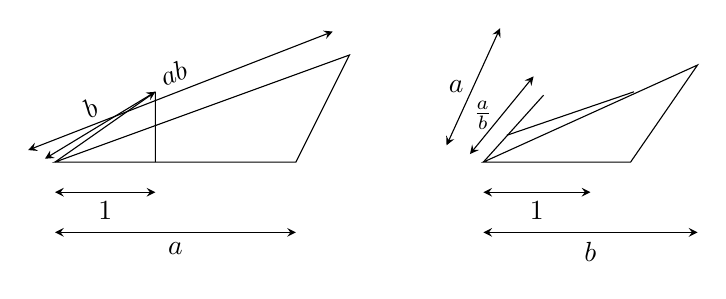
\begin{tikzpicture}[scale=0.85,>=stealth]
		% left construction: product
		\coordinate (A) at (0,0);
		\coordinate (B) at (3.6,0);
		\coordinate (C) at (4.4,1.6);
		\coordinate (D) at (1.5,1.05);
		\draw (A)--(B)--(C)--cycle;
		\draw (A)--(D);
		\draw (1.5,0)--(D);
		\draw[<->] (0,-0.45)--node[below]{$1$}(1.5,-0.45);
		\draw[<->] (0,-1.05)--node[below]{$a$}(3.6,-1.05);
		\draw[<->] (-0.15,0.05)--node[above,sloped]{$b$}(1.5,1.05);
		\draw[<->] (-0.4,0.18)--node[above,sloped]{$ab$}(4.15,1.95);
		% right construction: quotient
		\begin{scope}[xshift=6.4cm]
			\coordinate (A) at (0,0);
			\coordinate (B) at (2.2,0);
			\coordinate (C) at (3.2,1.45);
			\coordinate (D) at (0.9,1.0);
			\coordinate (E) at (0.35,0.4);
			\draw (A)--(B)--(C)--cycle;
			\draw (A)--(D);
			\draw (E)--(2.25,1.05);
			\draw[<->] (0,-0.45)--node[below]{$1$}(1.6,-0.45);
			\draw[<->] (0,-1.05)--node[below]{$b$}(3.2,-1.05);
			\draw[<->] (-0.2,0.12)--node[left]{$\frac ab$}(0.75,1.28);
			\draw[<->] (-0.55,0.25)--node[left]{$a$}(0.25,2.0);
		\end{scope}
	\end{tikzpicture}
	
	\textbf{图 1}
\end{center}

如果给定 $a$，则作出 $\sqrt a$ 也是一个初等几何作图：按图 2 所示，作直径为 $1+a$ 的圆，并在直径上作垂线。则 $\sqrt a$ 就是这条垂线的长度。

\begin{center}
	\begin{tikzpicture}[scale=1.0,>=stealth]
		\draw (0,0) arc (180:0:2.7 and 1.55);
		\draw (0,0)--(5.4,0);
		\coordinate (P) at (3.75,0);
		\coordinate (Q) at (3.75,1.45);
		\draw (P)--(Q);
		\draw[<->] ($(P)+(-0.28,0)$)--node[left]{$\sqrt a$}($(Q)+(-0.28,0)$);
		\draw[<->] (0,-0.18)--node[below]{$a$}(3.75,-0.18);
		\draw[<->] (3.75,-0.18)--node[below]{$1$}(5.4,-0.18);
	\end{tikzpicture}\qquad \textbf{图 2}
\end{center}

由此可知，直尺与圆规作图给出了实数中的加法、减法、乘法和除法（除以非零元素）这些全部代数运算，所以可作元素的全体是 $\mathbb R$ 的一个子域。还可以对可作元素开平方。我们现在将看到，这些本质上是仅有的可能操作。

由给定长度 $1$ 出发，通过这些操作可以作出所有有理数 $\mathbb Q$。因此我们可以作出所有坐标为有理数的点 $(x,y)\in\mathbb R^2$。通过开平方，我们可以作出 $\mathbb R$ 的附加元素，所以从 $1$ 出发可作的 $\mathbb R$ 的元素全体形成一个严格大于 $\mathbb Q$ 的域。

连接两个坐标在某个域 $F$ 中的点的直线的通常公式（“两点式”）给出直线的方程，其形式为
\[
ax+by-c=0,
\]
其中 $a,b,c\in F$。联立求解两个这样的方程以确定两条这样的直线的交点，所得解也在 $F$ 中。因此，如果两个点的坐标属于域 $F$，则仅用直尺作图不会产生坐标不也在 $F$ 中的额外点。

圆规作图（上面的类型 (3) 或 (4)）定义的是由一个圆与一条直线或另一个圆相交所得到的点。圆心为 $(h,k)$、半径为 $r$ 的圆有方程
\[
(x-h)^2+(y-k)^2=r^2,
\]
所以，当我们考虑圆规作图对域 $F$ 的元素的影响时，我们是在考虑这样的一个方程与一个线性方程
\[
ax+by-c=0
\]
的联立解，其中 $a,b,c,h,k,r\in F$，或者两个二次方程的联立解。

在线性方程与圆的方程的情形中，例如从线性方程中解出 $y$，并代入圆方程，会得到关于 $x$ 的二次方程（而 $y$ 由 $x$ 线性给出）。因此交点的坐标至多位于 $F$ 的一个二次扩张中。

在两个圆相交的情形中，设为
\[
(x-h)^2+(y-k)^2=r^2
\]
和
\[
(x-h')^2+(y-k')^2=r'^2,
\]
用第二个方程从第一个方程中相减，说明考虑下面两个方程会得到相同的交点：
\[
(x-h)^2+(y-k)^2=r^2
\]
以及
\[
2(h'-h)x+2(k'-k)y=r^2-h^2-k^2-r'^2+h'^2+k'^2,
\]
这正是前面所考虑类型的一个圆与一条直线的交点（事实上，这条直线连接两个交点）。

由此可知，如果给定一族可作元素，则可以作出由这些元素生成的 $\mathbb R$ 的子域 $F$ 中的所有元素；并且对 $F$ 的元素所作的任意直尺与圆规操作，所产生的元素至多位于 $F$ 的一个二次扩张中。由于二次扩张的次数为 $2$，且扩张次数是可乘的，因此如果 $\alpha\in\mathbb R$ 是由域 $F$ 中的元素经过一系列（有限个）直尺与圆规操作得到的，那么 $\alpha$ 属于 $F$ 的一个次数为 $2$ 的幂的扩张 $K$ 中：对某个 $m$，有
\[
[K:F]=2^m.
\]
由于 $[F(\alpha):F]$ 整除这个扩张次数，所以它也必须是 $2$ 的幂。

\noindent\textbf{命题 23.} 若元素 $\alpha\in\mathbb R$ 是由一个域 $F\subset\mathbb R$ 经由一系列圆规与直尺作图得到的，则对某个整数 $k\geq 0$，有
\[
[F(\alpha):F]=2^k.
\]

\noindent\textbf{定理 24.} 经典希腊问题：（I）倍立方体，（II）三等分角，以及（III）化圆为方，均不可能完成。

\begin{proof}
	（I）倍立方体等价于从单位 $1$ 出发在实数中作出 $\sqrt[3]{2}$。由于
	\[
	[\mathbb Q(\sqrt[3]{2}):\mathbb Q]=3
	\]
	不是 $2$ 的幂，这是不可能的。
	
	（II）如果一个角 $\theta$ 可作，那么在 $\mathbb R^2$ 中确定从原点出发、与正 $x$ 轴成角 $\theta$ 且距离为 $1$ 的点，说明 $\cos\theta$（该点的 $x$-坐标）可作（于是 $\sin\theta$ 也可作）。反过来，如果 $\cos\theta$，从而 $\sin\theta$，可作，则具有这些坐标的点给出角 $\theta$。
	
	于是三等分角 $\theta$ 的问题等价于如下问题：给定 $\cos\theta$，作出 $\cos(\theta/3)$。
	
	为说明这并非总是可能的（它当然有时是可能的，例如 $\theta=180^\circ$），考虑 $\theta=60^\circ$。于是 $\cos\theta=\frac12$。由余弦的三倍角公式：
	\[
	\cos\theta=4\cos^3(\theta/3)-3\cos(\theta/3),
	\]
	代入 $\theta=60^\circ$，可见 $\beta=\cos20^\circ$ 满足方程
	\[
	4\beta^3-3\beta-1/2=0,
	\]
	或者
	\[
	8\beta^3-6\beta-1=0.
	\]
	这可写成
	\[
	(2\beta)^3-3(2\beta)-1=0.
	\]
	令 $\alpha=2\beta$。则 $\alpha$ 是一个介于 $0$ 与 $2$ 之间的实数，并满足方程
	\[
	\alpha^3-3\alpha-1=0.
	\]
	但我们在上一节已经考察过这个方程，并确定 $[\mathbb Q(\alpha):\mathbb Q]=3$；同上可见 $\alpha$ 不可作。
	
	（III）化圆为方等价于确定实数
	\[
	\pi=3.14159\ldots
	\]
	是否可作。如前所述，甚至证明这个数不是有理数也是一个困难问题。事实上它是超越的（我们将不加证明地假设这一点），所以 $[\mathbb Q(\pi):\mathbb Q]$ 甚至不是有限的，更不可能是 $2$ 的幂，这说明用直尺与圆规化圆为方是不可能的。
\end{proof}

\paragraph{注记：} 上面的证明说明 $\cos20^\circ$ 和 $\sin20^\circ$ 不能作出。问题随之出现：哪些整数角（以度为单位测量）是可作的？角 $1^\circ$ 和 $2^\circ$ 不可作，因为否则正弦和余弦的加法公式将给出 $20^\circ$ 的可作性。另一方面，初等几何作图（作正五边形得到 $72^\circ$ 的角，作等边三角形得到 $60^\circ$ 的角）连同加法公式和半角公式说明 $\cos3^\circ$ 与 $\sin3^\circ$ 是可作的。由此可知，一个整数度角的三角函数可作，当且仅当这个角是 $3^\circ$ 的倍数。明确地，
\[
\cos 3^\circ
=\frac18(\sqrt3+1)\sqrt{5+\sqrt5}
+\frac1{16}(\sqrt6-\sqrt2)(\sqrt5-1)
\]
并且
\[
\sin 3^\circ
=\frac1{16}(\sqrt6+\sqrt2)(\sqrt5-1)
-\frac18(\sqrt3-1)\sqrt{5+\sqrt5},
\]
这说明它们是由 $\mathbb Q$ 经过连续开平方和域运算得到的。

在第 14.5 节讨论分圆域之后，我们将考虑另一个经典几何问题：“哪些正 $n$ 边形可以用直尺与圆规作出？”（参见命题 14.29）。

这里我们一直谨慎地考虑使用直尺而不是带刻度的尺子来作图，区别在于带刻度的尺子上有标记。如果使用带刻度的尺子，则可以作出许多附加的代数元素。例如，假设 $\theta$ 是一个给定角，并且单位距离 $1$ 被标在尺子上。如图 3 所示，作一个半径为 $1$、圆心角为 $\theta$ 的圆，然后滑动尺子，直到圆上点 $A$ 与 $B$ 之间的距离为 $1$。于是一些初等几何说明（参见练习），所示角 $\alpha$ 为 $\theta/3$，即这个构造（归功于 Archimedes）三等分 $\theta$。特别地，定理 24 中第二个经典问题（三等分角）可以用带刻度的尺子和圆规解决。

\begin{center}
	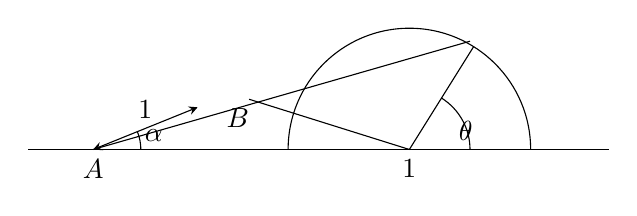
\begin{tikzpicture}[scale=1.1,>=stealth]
		\draw (-0.5,0)--(6.2,0);
		\coordinate (O) at (3.9,0);
		\draw (O) ++(-1.4,0) arc (180:0:1.4);
		\draw (O)--++(58:1.4);
		\draw (O)--++(-1.4,0);
		\coordinate (A) at (0.25,0);
		\coordinate (B) at (2.05,0.58);
		\coordinate (C) at (4.6,1.25);
		\draw (A)--(C);
		\draw (B)--(O);
		\draw[<->] (A)++(12:0.0)--node[above]{$1$}++(22:1.3);
		\draw (A) ++(0.55,0) arc (0:22:0.55);
		\node at (0.95,0.16) {$\alpha$};
		\draw (O) ++(0.7,0) arc (0:58:0.7);
		\node at (4.55,0.22) {$\theta$};
		\node at (1.92,0.36) {$B$};
		\node[below] at (A) {$A$};
		\node[below] at (O) {$1$};
	\end{tikzpicture}\qquad \textbf{图 3}
\end{center}

定理 24 中第一个经典问题（倍立方体），即作出 $\sqrt[3]{2}$，也可以用带刻度的尺子和圆规解决。下面给出对任意给定的正实数 $k<1$ 作出 $k^{1/3}$ 的构造。这个构造是 J. H. Conway 告诉我们的。

作半径为 $1$ 的圆，并以点 $A=(k,0)$ 为圆心，作出点
\[
B=(0,\sqrt{1-k^2}).
\]
把这个距离三等分，作出点
\[
(0,\tfrac13\sqrt{1-k^2}),
\]
并画出连接此点与 $A$ 的直线。滑动带有标记单位长度 $1$ 的尺子，使它经过点 $B$，并使从交点 $C$ 到它与 $x$-轴的交点 $D$ 的距离为 $1$，如图 4 所示。

于是 $A$ 与 $D$ 之间的距离为 $2k^{1/3}$，而 $B$ 与 $C$ 之间的距离为 $2k^{2/3}$（参见练习）。

\begin{center}
	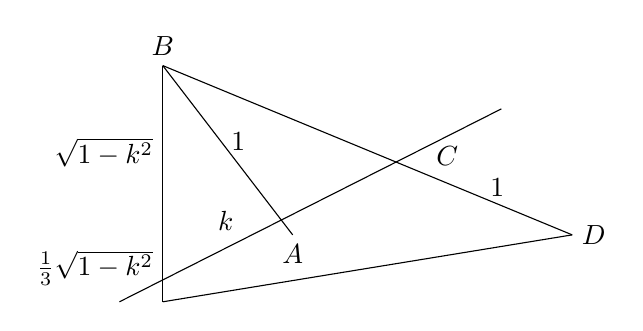
\begin{tikzpicture}[scale=1.0,>=stealth]
		\coordinate (B) at (0,3.0);
		\coordinate (A) at (1.65,0.85);
		\coordinate (C) at (3.35,1.85);
		\coordinate (D) at (5.2,0.85);
		\coordinate (E) at (0,0);
		\coordinate (F) at (0,0.85);
		\draw (E)--(D);
		\draw (E)--(B);
		\draw (B)--(D);
		\draw (A)--(B);
		\draw (-0.55,0.0)--(4.3,2.45);
		\node[above] at (B) {$B$};
		\node[below] at (A) {$A$};
		\node[right] at (C) {$C$};
		\node[right] at (D) {$D$};
		\node at (0.8,1.03) {$k$};
		\node at (0.96,2.04) {$1$};
		\node at (4.25,1.45) {$1$};
		\node[left] at (0,1.9) {$\sqrt{1-k^2}$};
		\node[left] at (0,0.43) {$\frac13\sqrt{1-k^2}$};
	\end{tikzpicture}\qquad \textbf{图 4}
\end{center}

\subsection*{练习}

\begin{enumerate}[label=\arabic*.]
	\item 证明不可能作出正九边形。
	
	\item 证明 Archimedes 的构造确实三等分角 $\theta$。\,[注意图 5 中的等腰三角形，以证明 $\beta=\gamma=2\alpha$。]
	
	\begin{center}
		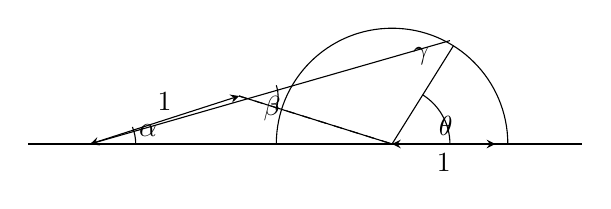
\begin{tikzpicture}[scale=1.05,>=stealth]
			\draw (-0.5,0)--(6.2,0);
			\coordinate (O) at (3.9,0);
			\draw (O) ++(-1.4,0) arc (180:0:1.4);
			\draw (O)--++(58:1.4);
			\coordinate (A) at (0.25,0);
			\coordinate (B) at (2.05,0.58);
			\coordinate (C) at (4.6,1.25);
			\draw (A)--(C);
			\draw (B)--(O);
			\draw[dashed] (B)--(O);
			\draw[<->] (A)--node[above]{$1$}(B);
			\draw[<->] (O)--node[below]{$1$}(5.15,0);
			\draw (A) ++(0.55,0) arc (0:22:0.55);
			\node at (0.95,0.16) {$\alpha$};
			\draw (B) ++(0.45,0.13) arc (18:-20:0.45);
			\node at (2.45,0.43) {$\beta$};
			\node at (4.25,1.06) {$\gamma$};
			\draw (O) ++(0.7,0) arc (0:58:0.7);
			\node at (4.55,0.22) {$\theta$};
		\end{tikzpicture}\qquad \textbf{图 5}
	\end{center}
	
	\item 证明文中所示 Conway 的构造确实作出了 $2k^{1/3}$ 和 $2k^{2/3}$。\,[一种方法：令 $(x,y)$ 为点 $C$ 的坐标，令 $a$ 为从 $B$ 到 $C$ 的距离，$b$ 为从 $A$ 到 $D$ 的距离；用相似三角形证明
	\[
	\text{(a)}\quad \frac{y}{1}=\frac{\sqrt{1-k^2}}{1+a},
	\]
	\[
	\text{(b)}\quad \frac{x}{a}=\frac{b+k}{1+a},
	\qquad
	\text{(c)}\quad \frac{y}{x-k}=\frac{\sqrt{1-k^2}}{3k},
	\]
	并且还证明
	\[
	\text{(d)}\quad (1-k^2)+(b+k)^2=(1+a)^2;
	\]
	解这些方程求出 $a$ 和 $b$。]
	
	\item 正七边形的构造等价于 $\cos(2\pi/7)$ 的可作性。我们以后将看到（第 14.5 节和第 14.7 节练习 2），
	\[
	\alpha=2\cos(2\pi/7)
	\]
	满足方程
	\[
	x^3+x^2-2x-1=0.
	\]
	利用这一点证明正七边形不能由直尺与圆规作出。
	
	\item 利用 $\alpha=2\cos(2\pi/5)$ 满足方程
	\[
	x^2+x-1=0
	\]
	这一事实，推出正五边形可以用直尺与圆规作出。
\end{enumerate}
\section{分裂域与代数闭包}

设 $F$ 是一个域。

若 $f(x)$ 是 $F[x]$ 中的任意多项式，则我们已经在第 2 节看到，存在一个域 $K$，它可以（通过把 $F$ 与 $F$ 的一个同构副本等同起来）看作 $F$ 的一个扩张，并且在其中 $f(x)$ 有一个根 $\alpha$。这等价于说 $f(x)$ 在 $K[x]$ 中有一个线性因子 $x-\alpha$（这是第 9 章命题 9）。

\noindent\textbf{定义.} 域 $F$ 的扩域 $K$ 称为多项式 $f(x)\in F[x]$ 的一个\emph{分裂域}，如果 $f(x)$ 在 $K[x]$ 中完全分解为线性因子（或称在 $K[x]$ 中完全分裂），并且 $f(x)$ 不在任何含有 $F$ 的 $K$ 的真子域上完全分解为线性因子。


若 $f(x)$ 的次数为 $n$，则 $f(x)$ 在 $F$ 中至多有 $n$ 个根（第 9 章命题 17），并且当且仅当 $f(x)$ 在 $F[x]$ 中完全分裂时，$f(x)$ 在 $F$ 中恰有 $n$ 个根（按重数计）。

\noindent\textbf{定理 25.} 对任意域 $F$，若 $f(x)\in F[x]$，则存在 $F$ 的一个扩张 $K$，它是 $f(x)$ 的分裂域。


\begin{proof}
	我们首先对 $f(x)$ 的次数 $n$ 用归纳法证明：存在 $F$ 的一个扩张 $E$，在它上面 $f(x)$ 完全分解为线性因子。若 $n=1$，则取 $E=F$。现在设 $n>1$。若 $f(x)$ 在 $F$ 上的不可约因子全都为次数 $1$，则 $F$ 就是 $f(x)$ 的分裂域，因而可取 $E=F$。否则，$f(x)$ 在 $F[x]$ 中至少有一个不可约因子，比如 $p(x)$，次数至少为 $2$。由定理 3，存在 $F$ 的一个扩张 $E_1$，它含有 $p(x)$ 的一个根 $\alpha$。在 $E_1$ 上，多项式 $f(x)$ 有线性因子 $x-\alpha$。$f(x)$ 的其余因子 $f_1(x)$ 的次数为 $n-1$，所以由归纳假设，存在 $E_1$ 的一个扩张 $E$，它含有 $f_1(x)$ 的全部根。由于 $\alpha\in E$，$E$ 是 $F$ 的一个扩张，且含有 $f(x)$ 的全部根。现在令 $K$ 为 $E$ 的所有含有 $F$ 且同时含有 $f(x)$ 全部根的子域的交。则 $K$ 是一个域，并且是 $f(x)$ 的分裂域。
\end{proof}

我们很快将看到，$f(x)$ 的任意两个分裂域都是同构的（这推广了定理 8），所以我们常常（滥用语言地）说一个多项式的\emph{这个}分裂域。

\noindent\textbf{定义.} 若 $K$ 是 $F$ 的代数扩张，并且 $K$ 是 $F$ 上一族多项式 $f(x)\in F[x]$ 的分裂域，则称 $K$ 是 $F$ 的一个\emph{正规扩张}。


我们通常使用术语“分裂域”而不是“正规扩张”（也见第 14.9 节）。


	\begin{enumerate}[label=(\arabic*)]
		\item $x^2-2$ 在 $\mathbb Q$ 上的分裂域正是 $\mathbb Q(\sqrt2)$，因为两个根是 $\pm\sqrt2$，而 $-\sqrt2\in\mathbb Q(\sqrt2)$。
		
		\item $(x^2-2)(x^2-3)$ 的分裂域是由 $\sqrt2$ 和 $\sqrt3$ 在 $\mathbb Q$ 上生成的域 $\mathbb Q(\sqrt2,\sqrt3)$，因为该多项式的根是 $\pm\sqrt2,\pm\sqrt3$。我们已经看到，这是 $\mathbb Q$ 上次数为 $4$ 的扩张，并且有如下已知子域图：
		
		\begin{center}
			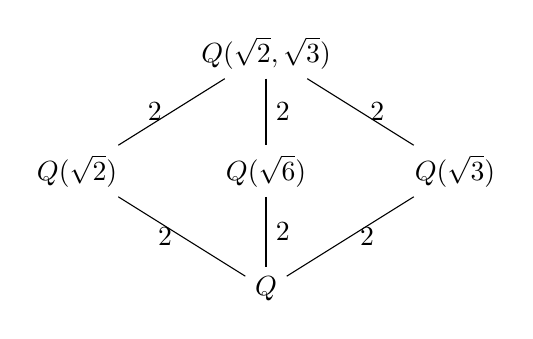
\begin{tikzpicture}[scale=1.0,>=stealth]
				\node (top) at (0,3) {$\mathbb Q(\sqrt2,\sqrt3)$};
				\node (l) at (-2.4,1.5) {$\mathbb Q(\sqrt2)$};
				\node (m) at (0,1.5) {$\mathbb Q(\sqrt6)$};
				\node (r) at (2.4,1.5) {$\mathbb Q(\sqrt3)$};
				\node (bot) at (0,0) {$\mathbb Q$};
				\draw (top)--node[left]{$2$}(l);
				\draw (top)--node[right]{$2$}(m);
				\draw (top)--node[right]{$2$}(r);
				\draw (l)--node[left]{$2$}(bot);
				\draw (m)--node[right]{$2$}(bot);
				\draw (r)--node[right]{$2$}(bot);
			\end{tikzpicture}
		\end{center}
		
		\item $x^3-2$ 在 $\mathbb Q$ 上的分裂域不只是 $\mathbb Q(\sqrt[3]{2})$，因为如前面指出的，这个多项式在 $\mathbb C$ 中的三个根是
		\[
		\sqrt[3]{2},\qquad
		\sqrt[3]{2}\left(\frac{-1+i\sqrt3}{2}\right),\qquad
		\sqrt[3]{2}\left(\frac{-1-i\sqrt3}{2}\right),
		\]
		而后两个根不是 $\mathbb Q(\sqrt[3]{2})$ 的元素，因为这个域的元素形如 $a+b\sqrt[3]{2}+c\sqrt[3]{4}$，其中 $a,b,c$ 为有理数，并且所有这样的数都是实数。
		
		该多项式的分裂域 $K$ 由把这三个根全部添加到 $\mathbb Q$ 中得到。注意，由于 $K$ 含有上面前两个根，所以它含有它们的商
		\[
		\frac{-1+\sqrt{-3}}{2},
		\]
		从而 $K$ 含有元素 $\sqrt{-3}$。另一方面，任意含有 $\sqrt[3]{2}$ 和 $\sqrt{-3}$ 的域都含有上面三个根。因此
		\[
		K=\mathbb Q(\sqrt[3]{2},\sqrt{-3})
		\]
		是 $x^3-2$ 在 $\mathbb Q$ 上的分裂域。因为 $\sqrt{-3}$ 满足方程 $x^2+3=0$，这个扩张在 $\mathbb Q(\sqrt[3]{2})$ 上的次数至多为 $2$；又由于我们上面观察到 $\mathbb Q(\sqrt[3]{2})$ 不是分裂域，所以次数必为 $2$。于是
		\[
		[\mathbb Q(\sqrt[3]{2},\sqrt{-3}):\mathbb Q]=6.
		\]
		注意，我们也可以在最后略有不同地进行：指出 $\mathbb Q(\sqrt{-3})$ 是 $K$ 的一个子域，于是指数 $[\mathbb Q(\sqrt{-3}):\mathbb Q]=2$ 整除 $[K:\mathbb Q]$。由于这个扩张次数还被 $3$ 整除（因为 $\mathbb Q(\sqrt[3]{2})\subset K$），次数被 $6$ 整除，因此必为 $6$。
		
		这给出了如下已知子域图：
		\begin{center}
			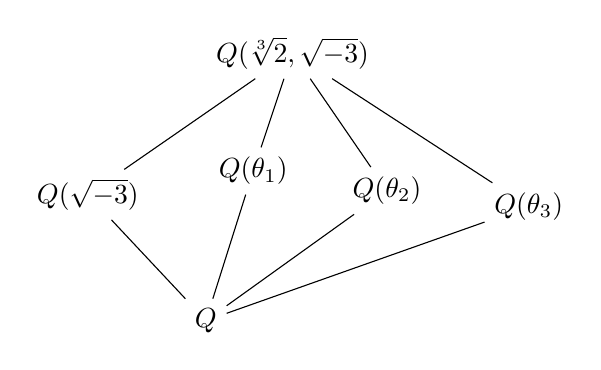
\begin{tikzpicture}[scale=1.0]
				\node (top) at (0,3.4) {$\mathbb Q(\sqrt[3]{2},\sqrt{-3})$};
				\node (qneg) at (-2.6,1.6) {$\mathbb Q(\sqrt{-3})$};
				\node (q1) at (-0.5,1.9) {$\mathbb Q(\theta_1)$};
				\node (q2) at (1.2,1.65) {$\mathbb Q(\theta_2)$};
				\node (q3) at (3.0,1.45) {$\mathbb Q(\theta_3)$};
				\node (bot) at (-1.1,0) {$\mathbb Q$};
				\draw (top)--(qneg);
				\draw (top)--(q1);
				\draw (top)--(q2);
				\draw (top)--(q3);
				\draw (qneg)--(bot);
				\draw (q1)--(bot);
				\draw (q2)--(bot);
				\draw (q3)--(bot);
			\end{tikzpicture}
		\end{center}
		其中
		\[
		\theta_1=\sqrt[3]{2},\qquad
		\theta_2=\sqrt[3]{2}\left(\frac{-1+i\sqrt3}{2}\right),\qquad
		\theta_3=\sqrt[3]{2}\left(\frac{-1-i\sqrt3}{2}\right).
		\]
		
		\item 在计算分裂域时必须小心。多项式 $x^4+4$ 在 $\mathbb Q$ 上的分裂域比起初可能猜想的更小。事实上，这个多项式在 $\mathbb Q$ 上分解为
		\begin{align*}
			x^4+4 &= x^4+4x^2+4-4x^2 \\
			&=(x^2+2)^2-4x^2 \\
			&=(x^2+2x+2)(x^2-2x+2),
		\end{align*}
		其中这两个因子不可约（又由 Eisenstein 判别法）。用二次公式求解这两个因子的根，我们得到四个根
		\[
		\pm1\pm i,
		\]
		所以这个多项式的分裂域只是域 $\mathbb Q(i)$，它是 $\mathbb Q$ 的次数为 $2$ 的扩张。
	\end{enumerate}


一般地，若 $f(x)\in F[x]$ 是次数为 $n$ 的多项式，则向 $F$ 添加 $f(x)$ 的一个根会生成次数至多为 $n$ 的扩张 $F_1$（并且当且仅当 $f(x)$ 不可约时次数等于 $n$）。在 $F_1$ 上，多项式 $f(x)$ 现在至少有一个线性因子，所以 $f(x)$ 的任何另一个根都在 $F_1$ 上满足一个次数至多为 $n-1$ 的方程。把这样一个根添加到 $F_1$ 中，于是得到 $F_1$ 的一个次数至多为 $n-1$ 的扩张，等等。利用扩张次数的可乘性，这证明了

\noindent\textbf{命题 26.} 一个次数为 $n$ 的多项式在 $F$ 上的分裂域在 $F$ 上的次数至多为 $n!$。


如上面的例子所示，分裂域的次数可能小于 $n!$。以后将用 Galois 理论证明，$\mathbb Q$ 上次数为 $n$ 的“通常”多项式（在一个明确定义的意义下）的分裂域次数为 $n!$，所以这可看作“典型”情形（虽然我们将考虑的大多数有趣例子的分裂域次数更小）。

\paragraph{例（$x^n-1$ 的分裂域：分圆域）}
考虑多项式 $x^n-1$ 在 $\mathbb Q$ 上的分裂域。这个多项式的根称为 $n$ 次单位根。
	
	回忆每个非零复数 $a+bi\in\mathbb C$ 都能唯一写成
	\[
	re^{i\theta}=r(\cos\theta+i\sin\theta),\qquad r>0,
	\quad 0\leq \theta<2\pi,
	\]
	这不过是在复平面中用极坐标表示点 $a+bi$：$r$ 是 $(a,b)$ 到原点的距离，$\theta$ 是与正实轴所成的角。
	
	在 $\mathbb C$ 上，方程 $x^n=1$ 有 $n$ 个不同的解，即元素
	\[
	e^{2\pi k i/n}=\cos\left(\frac{2\pi k}{n}\right)+i\sin\left(\frac{2\pi k}{n}\right)
	\]
	其中 $k=0,1,\ldots,n-1$。在几何上，这些点是在复平面中半径为 $1$ 的圆上从点 $(1,0)$（对应 $k=0$）开始的 $n$ 个等距点（见图 6）。这些数全都是 $n$ 次单位根这一事实是立即的，因为
	\[
	\left(e^{2\pi k i/n}\right)^n=e^{(2\pi k i/n)n}=e^{2\pi k i}=1.
	\]
	于是 $\mathbb C$ 含有 $x^n-1$ 的一个分裂域，而且我们常常把 $x^n-1$ 在 $\mathbb Q$ 上的分裂域看作在 $\mathbb C$ 中由上面的数在 $\mathbb Q$ 上生成的域。
	
	\begin{center}
		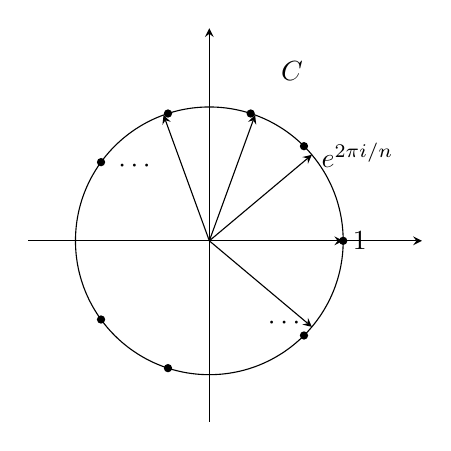
\begin{tikzpicture}[scale=1.0,>=stealth]
			\draw[->] (-2.3,0)--(2.7,0);
			\draw[->] (0,-2.3)--(0,2.7);
			\draw (0,0) circle (1.7);
			\foreach \ang in {0,45,72,108,144,216,252,315}{
				\fill ({1.7*cos(\ang)},{1.7*sin(\ang)}) circle (1.5pt);
			}
			\draw[->] (0,0)--(1.7,0) node[right]{$1$};
			\draw[->] (0,0)--({1.7*cos(40)},{1.7*sin(40)}) node[right]{$e^{2\pi i/n}$};
			\draw[->] (0,0)--({1.7*cos(70)},{1.7*sin(70)});
			\draw[->] (0,0)--({1.7*cos(110)},{1.7*sin(110)});
			\draw[->] (0,0)--({1.7*cos(-40)},{1.7*sin(-40)});
			\node at (1.05,2.15) {$\mathbb C$};
			\node at (-0.95,0.95) {$\cdots$};
			\node at (0.95,-1.05) {$\cdots$};
		\end{tikzpicture}
		
		\textbf{图 6}
	\end{center}
	
	在 $x^n-1$ 的任意抽象分裂域 $K/\mathbb Q$ 中，$n$ 次单位根全体在乘法下形成一个群，因为若 $\alpha^n=1$ 且 $\beta^n=1$，则 $(\alpha\beta)^n=1$，所以 $K^\times$ 的这个子集在乘法下封闭。由此可知这是一个循环群（第 9 章命题 18）；我们将看到在 $K$ 中有 $n$ 个不同的根，所以它的阶为 $n$。
	
	\noindent\textbf{定义.} 全体 $n$ 次单位根所成循环群的一个生成元称为一个\emph{本原 $n$ 次单位根}。

	
	令 $\zeta_n$ 表示一个本原 $n$ 次单位根。于是其他本原 $n$ 次单位根是元素 $\zeta_n^a$，其中 $1\leq a<n$ 是与 $n$ 互素的整数，因为这些正是阶为 $n$ 的循环群的其他生成元。特别地，恰有 $\varphi(n)$ 个本原 $n$ 次单位根，其中 $\varphi(n)$ 表示 Euler $\varphi$-函数。
	
	在 $\mathbb C$ 上，我们可以直接看出这一切：令
	\[
	\zeta_n=e^{2\pi i/n}
	\]
	（即从 $1$ 出发逆时针方向遇到的第一个 $n$ 次单位根）。于是所有其他单位根都是 $\zeta_n$ 的幂：
	\[
	e^{2\pi k i/n}=\zeta_n^k,
	\]
	所以 $\zeta_n$ 是 $n$ 次单位根乘法群的一个可能生成元。当我们在 $\mathbb C$ 中看单位根时，通常用 $\zeta_n$ 表示这个本原 $n$ 次单位根的选择。对若干小的 $n$，$\mathbb C$ 中的本原单位根为
	\[
	\zeta_1=1,
	\]
	\[
	\zeta_2=-1,
	\]
	\[
	\zeta_3=\frac{-1+i\sqrt3}{2},
	\]
	\[
	\zeta_4=i,
	\]
	\[
	\zeta_5=\frac{\sqrt5-1}{4}+i\left(\frac{\sqrt{10+2\sqrt5}}{4}\right),
	\]
	\[
	\zeta_6=\frac{1+i\sqrt3}{2},
	\]
	\[
	\zeta_8=\frac{\sqrt2}{2}+i\frac{\sqrt2}{2}
	\]
	（这些公式来自 $n$ 边形的初等几何；无论如何，通过把它们升到相应幂次可以直接验证）。
	
	$x^n-1$ 在 $\mathbb Q$ 上的分裂域是域 $\mathbb Q(\zeta_n)$，这个域有一个名称：
	
	\noindent\textbf{定义.} 域 $\mathbb Q(\zeta_n)$ 称为 $n$ 次单位根的\emph{分圆域}。

	
	确定这个扩张的次数需要分析 $\zeta_n$ 在 $\mathbb Q$ 上的极小多项式，并将推迟到后面（第 6 节）。我们事实上已经考虑过一个重要特例：$n=p$ 为素数。在这种情形下，我们有因式分解
	\[
	x^p-1=(x-1)(x^{p-1}+x^{p-2}+\cdots+x+1),
	\]
	并且由于 $\zeta_p\ne 1$，可知 $\zeta_p$ 是多项式
	\[
	\Phi_p(x)=\frac{x^p-1}{x-1}=x^{p-1}+x^{p-2}+\cdots+x+1
	\]
	的一个根；我们在第 9.4 节证明过这个多项式不可约。于是 $\Phi_p(x)$ 是 $\zeta_p$ 在 $\mathbb Q$ 上的极小多项式，所以
	\[
	[\mathbb Q(\zeta_p):\mathbb Q]=p-1.
	\]
	我们以后将看到，一般地 $[\mathbb Q(\zeta_n):\mathbb Q]=\varphi(n)$，其中 $\varphi(n)$ 是 $n$ 的 Euler phi-函数（因此 $\varphi(p)=p-1$）。


\paragraph{例（$x^p-2$ 的分裂域，$p$ 为素数）}
令 $p$ 为素数，并考虑 $x^p-2$ 的分裂域。若 $\alpha$ 是这个方程的一个根，即 $\alpha^p=2$，则 $(\zeta\alpha)^p=2$，其中 $\zeta$ 是任意 $p$ 次单位根。因此这个方程的解为
	\[
	\zeta\sqrt[p]{2},\qquad \zeta\text{ 是一个 }p\text{ 次单位根},
	\]
	其中照例，如果我们想把这些元素看作复数，符号 $\sqrt[p]{2}$ 表示 $2$ 的正实 $p$ 次根；而如果抽象地看待这些根，则它表示 $x^p=2$ 的任意一个解。由于两个解 $\zeta_p\sqrt[p]{2}$ 与 $\sqrt[p]{2}$ 的比正是 $\zeta_p$，其中 $\zeta_p$ 为一个本原 $p$ 次单位根，$x^p-2$ 在 $\mathbb Q$ 上的分裂域含有 $\mathbb Q(\sqrt[p]{2},\zeta_p)$。另一方面，上述所有根都在这个域中，所以分裂域恰为
	\[
	\mathbb Q(\sqrt[p]{2},\zeta_p).
	\]
	
	这个域含有 $p$ 次单位根的分圆域，并由 $\sqrt[p]{2}$ 在它上面生成，所以它是在该分圆域上的次数至多为 $p$ 的扩张。于是它在 $\mathbb Q$ 上的次数 $\leq p(p-1)$。由于 $\mathbb Q(\sqrt[p]{2})$ 和 $\mathbb Q(\zeta_p)$ 都是子域，所以这个扩张在 $\mathbb Q$ 上的次数同时被 $p$ 和 $p-1$ 整除。由于这两个数互素，扩张次数被 $p(p-1)$ 整除，所以必有
	\[
	[\mathbb Q(\sqrt[p]{2},\zeta_p):\mathbb Q]=p(p-1)
	\]
	（这是推论 22）。特别注意，我们已经证明 $x^p-2$ 在 $\mathbb Q(\zeta_p)$ 上仍不可约，这一点完全不是显然的。我们有如下已知子域图：
	\begin{center}
		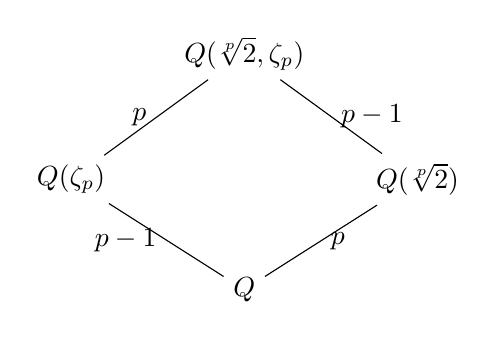
\begin{tikzpicture}[scale=1.0]
			\node (top) at (0,3) {$\mathbb Q(\sqrt[p]{2},\zeta_p)$};
			\node (left) at (-2.2,1.4) {$\mathbb Q(\zeta_p)$};
			\node (right) at (2.2,1.4) {$\mathbb Q(\sqrt[p]{2})$};
			\node (bot) at (0,0) {$\mathbb Q$};
			\draw (top)--node[left]{$p$}(left);
			\draw (top)--node[right]{$p-1$}(right);
			\draw (left)--node[left]{$p-1$}(bot);
			\draw (right)--node[right]{$p$}(bot);
		\end{tikzpicture}
	\end{center}
	
	特例 $p=3$ 正是上面的例 3，在那里我们只是把 $3$ 次单位根显式写了出来。


现在回到证明如下问题：多项式 $f(x)$ 在域 $F$ 上的分裂域如何构造并无差别。如定理 8 中那样，把结果表述为两个域之间的任意同构 $\varphi:F\overset{\sim}{\longrightarrow}F'$ 是方便的。

\noindent\textbf{定理 27.} 设 $\varphi:F\overset{\sim}{\longrightarrow}F'$ 是域的同构。设 $f(x)\in F[x]$ 是多项式，且 $f'(x)\in F'[x]$ 是把 $\varphi$ 作用到 $f(x)$ 的系数上所得到的多项式。设 $E$ 是 $f(x)$ 在 $F$ 上的分裂域，$E'$ 是 $f'(x)$ 在 $F'$ 上的分裂域。则同构 $\varphi$ 可扩张为一个同构 $\sigma:E\overset{\sim}{\longrightarrow}E'$，即 $\sigma$ 限制到 $F$ 上就是同构 $\varphi$：
	\[
	\begin{array}{ccc}
		\sigma:E&\longrightarrow&E'\\
		& & \\
		\varphi:F&\longrightarrow&F'.
	\end{array}
	\]


\begin{proof}
	我们对 $f(x)$ 的次数 $n$ 归纳。如定理 8 前的讨论所说，回忆从一个域 $F$ 到另一个域 $F'$ 的同构 $\varphi$ 在多项式环 $F[x]$ 与 $F'[x]$ 之间诱导一个自然同构。特别地，若 $f(x)$ 和 $f'(x)$ 在这个同构下相互对应，则 $f(x)$ 在 $F[x]$ 中的不可约因子对应于 $f'(x)$ 在 $F'[x]$ 中的不可约因子。
	
	若 $f(x)$ 的全部根都在 $F$ 中，则 $f(x)$ 在 $F[x]$ 中完全分裂，并且 $f'(x)$ 在 $F'[x]$ 中完全分裂（其线性因子就是 $f(x)$ 的线性因子的像）。因此 $E=F$ 且 $E'=F'$，在这种情形可取 $\sigma=\varphi$。这说明对 $n=1$ 以及 $f(x)$ 的全部不可约因子都次数为 $1$ 的情形，结果成立。
	
	现在假设归纳地，定理已对任意域 $F$、同构 $\varphi$ 以及次数小于 $n$ 的多项式 $f(x)\in F[x]$ 得到证明。令 $p(x)$ 为 $f(x)$ 在 $F[x]$ 中次数至少为 $2$ 的一个不可约因子，令 $p'(x)$ 为 $f'(x)$ 在 $F'[x]$ 中相应的不可约因子。若 $\alpha\in E$ 是 $p(x)$ 的一个根，且 $\beta\in E'$ 是 $p'(x)$ 的一个根，则由定理 8，我们可以把 $\varphi$ 扩张为一个同构 $\sigma':F(\alpha)\overset{\sim}{\longrightarrow}F'(\beta)$：
	\[
	\begin{array}{ccc}
		\sigma':F(\alpha)&\longrightarrow&F'(\beta)\\
		& & \\
		\varphi:F&\longrightarrow&F'.
	\end{array}
	\]
	令 $F_1=F(\alpha)$，$F'_1=F'(\beta)$，于是有同构 $\sigma':F_1\overset{\sim}{\longrightarrow}F'_1$。在 $F_1$ 上我们有 $f(x)=(x-\alpha)f_1(x)$，其中 $f_1(x)$ 次数为 $n-1$，并且 $f'(x)=(x-\beta)f'_1(x)$。域 $E$ 是 $f_1(x)$ 在 $F_1$ 上的一个分裂域：$f_1(x)$ 的所有根都在 $E$ 中，并且若它们包含在任何更小的含有 $F_1$ 的扩张 $L$ 中，那么由于 $F_1$ 含有 $\alpha$，$L$ 也将含有 $f(x)$ 的全部根，这将与 $E$ 作为 $f(x)$ 在 $F$ 上的分裂域的极小性矛盾。类似地，$E'$ 是 $f'_1(x)$ 在 $F'_1$ 上的一个分裂域。由于 $f_1(x)$ 与 $f'_1(x)$ 的次数都小于 $n$，由归纳假设，存在一个映射 $\sigma:E\overset{\sim}{\longrightarrow}E'$，它扩张同构 $\sigma':F_1\overset{\sim}{\longrightarrow}F'_1$。这给出扩张后的图：
	\[
	\begin{array}{ccccc}
		\sigma:E&\longrightarrow&E'\\
		& & \\
		\sigma':F_1&\longrightarrow&F'_1\\
		& & \\
		\varphi:F&\longrightarrow&F'.
	\end{array}
	\]
	于是，如图所示，$\sigma$ 限制到 $F_1$ 上就是同构 $\sigma'$，所以特别地，$\sigma$ 限制到 $F$ 上就是 $\sigma'$ 限制到 $F$ 上，也就是 $\varphi$，这说明 $\sigma$ 是 $\varphi$ 的一个扩张，证明完成。
\end{proof}

\noindent\textbf{推论 28（分裂域的唯一性）.} 域 $F$ 上一个多项式 $f(x)\in F[x]$ 的任意两个分裂域都是同构的。


\begin{proof}
	取 $\varphi$ 为从 $F$ 到自身的恒等映射，并取 $E$ 和 $E'$ 为 $f(x)(=f'(x))$ 的两个分裂域。
\end{proof}

如前所述，这个结果证明了“$f(x)$ 在 $F$ 上的分裂域”这一术语的合理性，因为任意两个这样的域都是同构的。分裂域在代数元素的研究中扮演自然的角色（如果你要添加一个多项式的一个根，为什么不添加全部根呢？），因此在 Galois 理论中占有特别重要的地位。

我们以讨论 $F$ 的那些含有 $F$ 上所有多项式的所有根的域扩张来结束本节。

\noindent\textbf{定义.} 若 $\overline F$ 是 $F$ 的代数扩张，并且每个 $f(x)\in F[x]$ 都在 $\overline F$ 上完全分裂（因而可说 $\overline F$ 含有 $F$ 上全部代数元素），则称域 $\overline F$ 是 $F$ 的一个\emph{代数闭包}。


\noindent\textbf{定义.} 若每个以 $K$ 中元素为系数的多项式都在 $K$ 中有一个根，则称域 $K$ 是\emph{代数闭的}。


代数闭域的存在并不显然，给定域 $F$ 的代数闭包存在也不显然（我们很快证明这一点）。

注意，若 $K$ 是代数闭的，则事实上每个 $f(x)\in K[x]$ 的全部根都在 $K$ 中，因为按定义 $f(x)$ 在 $K$ 中有一个根 $\alpha$，因而在 $K[x]$ 中有因子 $x-\alpha$。$f(x)$ 的余下因子于是仍是 $K[x]$ 中的一个多项式，所以也有一个根，因而又有一个线性因子，依此类推，所以 $f(x)$ 必完全分裂。因此，若 $K$ 是代数闭的，则 $K$ 本身就是 $K$ 的一个代数闭包；反过来则显然，所以 $K=\overline K$ 当且仅当 $K$ 是代数闭的。

下一个结果说明，“取代数闭包”的过程事实上一步就停止——取一个代数闭包的代数闭包不会给出更大的域：这个域已经是代数闭的（记号上：$\overline{\overline F}=\overline F$）。

\noindent\textbf{命题 29.} 设 $\overline F$ 是 $F$ 的一个代数闭包。则 $\overline F$ 是代数闭的。


\begin{proof}
	设 $f(x)$ 是 $\overline F[x]$ 中的一个多项式，并令 $\alpha$ 是 $f(x)$ 的一个根。于是 $\alpha$ 生成 $\overline F$ 的一个代数扩张 $\overline F(\alpha)$，而 $\overline F$ 在 $F$ 上代数。由定理 20，$\overline F(\alpha)$ 在 $F$ 上代数，所以特别地，其元素 $\alpha$ 在 $F$ 上代数。但于是 $\alpha\in\overline F$，说明 $\overline F$ 是代数闭的。
\end{proof}

给定一个域 $F$，我们已经证明了如何构造（有限）扩张，使其含有任意给定多项式 $f(x)\in F[x]$ 的全部根。直观地，$F$ 的一个代数闭包由所有这些域“生成”。这里的困难在于“生成”在哪里进行，因为它们并不全是某一个给定域的子域。对于有限个多项式 $f_1(x),\ldots,f_k(x)$，我们可以把它们的分裂域看作乘积多项式 $f_1(x)\cdots f_k(x)$ 的分裂域的子域；但同样的想法用于无限多个多项式时，需要大量“记账”式的等同以及 Zorn 引理的一次应用。

我们将换一种方式构造 $F$ 的一个代数闭包：先构造一个含有 $F$ 的代数闭域。证明使用 Artin 的一个巧妙想法：通过为每个多项式引入一个单独变量，非常简洁地解决了构造一个含有适当多项式根的域时的“记账”问题（这最终也依赖于 Zorn 引理）。

\noindent\textbf{命题 30.} 对任意域 $F$，存在一个含有 $F$ 的代数闭域 $K$。


\begin{proof}
	对每个以 $F$ 中元素为系数的非常数首一多项式 $f=f(x)$，令 $x_f$ 表示一个不定元，并考虑由这些变量 $x_f$ 在 $F$ 上生成的多项式环 $F[\ldots,x_f,\ldots]$。在这个多项式环中，考虑由多项式 $f(x_f)$ 生成的理想 $I$。若这个理想不是真理想，则 $1$ 是这个理想的一个元素，因而有一个关系
	\[
	g_1 f_1(x_{f_1})+g_2 f_2(x_{f_2})+\cdots+g_n f_n(x_{f_n})=1,
	\]
	其中 $g_i$，$i=1,2,\ldots,n$，是关于 $x_f$ 的多项式。对 $i=1,2,\ldots,n$，令 $x_{f_i}=x_i$，并令 $x_{n+1},\ldots,x_m$ 为多项式 $g_j$，$j=1,2,\ldots,n$ 中出现的其余变量。于是上面的关系写为
	\[
	g_1(x_1,x_2,\ldots,x_m)f_1(x_1)+\cdots+g_n(x_1,x_2,\ldots,x_m)f_n(x_n)=1.
	\]
	令 $F'$ 为 $F$ 的一个有限扩张，它含有 $f_i(x)$ 的一个根 $\alpha_i$，$i=1,2,\ldots,n$。在上面的多项式方程中令 $x_i=\alpha_i$，$i=1,2,\ldots,n$，并令 $x_{n+1}=\cdots=x_m=0$，比如说，就会推出 $F'$ 中 $0=1$，这显然不可能。
	
	既然理想 $I$ 是真理想，它包含于某个极大理想 $M$ 中（这正是使用 Zorn 引理之处）。于是商
	\[
	K_1=F[\ldots,x_f,\ldots]/M
	\]
	是一个含有 $F$（的一个同构副本）的域。由构造，每个多项式 $f$ 在 $K_1$ 中都有一个根，即 $x_f$ 的像，因为 $f(x_f)\in I\subseteq M$。我们已经构造了一个域 $K_1$，在其中每个系数来自 $F$ 的多项式都有一个根。
	
	用 $K_1$ 代替 $F$ 进行同样构造，得到一个含有 $K_1$ 的域 $K_2$，在其中所有系数来自 $K_1$ 的多项式都有一个根。如此继续，我们得到一列域
	\[
	F=K_0\subseteq K_1\subseteq K_2\subseteq\cdots\subseteq K_j\subseteq K_{j+1}\subseteq\cdots
	\]
	其中每个系数在 $K_j$ 中的多项式在 $K_{j+1}$ 中都有一个根，$j=0,1,\ldots$。令
	\[
	K=\bigcup_{j\geq 0}K_j
	\]
	为这些域的并。则 $K$ 显然是一个含有 $F$ 的域。由于 $K$ 是这些域 $K_j$ 的并，$K[x]$ 中任意多项式 $h(x)$ 的全部系数都属于某个 $K_N$，只要 $N$ 充分大。但于是 $h(x)$ 在 $K_{N+1}$ 中有一个根，所以在 $K$ 中有一个根。因此 $K$ 是代数闭的，证明完成。
\end{proof}

现在我们用含有 $F$ 的代数闭域来构造 $F$ 的一个代数闭包：

\noindent\textbf{命题 31.} 设 $K$ 是一个代数闭域，且 $F$ 是 $K$ 的一个子域。则 $K$ 中在 $F$ 上代数的元素全体 $\overline F$ 是 $F$ 的一个代数闭包。$F$ 的代数闭包在同构意义下唯一。


\begin{proof}
	按定义，$\overline F$ 是 $F$ 的一个代数扩张。每个多项式 $f(x)\in F[x]$ 在 $K$ 上完全分解为线性因子 $x-\alpha$（甚至 $K[x]$ 中的每个多项式也是如此）。但每个 $\alpha$ 都是 $f(x)$ 的一个根，所以在 $F$ 上代数，因而是 $\overline F$ 的一个元素。于是所有线性因子 $x-\alpha$ 的系数都在 $\overline F$ 中，即 $f(x)$ 在 $\overline F[x]$ 中完全分裂，$\overline F$ 是 $F$ 的一个代数闭包。
	
	代数闭包的唯一性（在同构意义下）鉴于分裂域的唯一性是自然的；它沿着同样的思路并配合 Zorn 引理的一次应用来证明，这里省略。
\end{proof}

我们以后将用 Galois 理论证明下面的结果（也存在使用复分析的纯解析证明）。

\noindent\textbf{定理（代数学基本定理）.} 域 $\mathbb C$ 是代数闭的。


由命题 31，我们立即得到：

\noindent\textbf{推论 32.} 域 $\mathbb C$ 含有它任一子域的代数闭包。特别地，$\overline{\mathbb Q}$，即 $\mathbb C$ 中在 $\mathbb Q$ 上代数的复数全体，是 $\mathbb Q$ 的一个代数闭包。


这些考虑的要点是：涉及域 $F$ 上代数元素的所有计算，都可以看作发生在一个（大的）域中，即 $\overline F$。类似地，我们可以有意义地谈论任意一族代数扩张的复合，只要把它们全都看作代数闭包的子域。在 $\mathbb Q$ 或 $\mathbb Q$ 的有限扩张的情形下，我们可以把所有计算都看作发生在 $\mathbb C$ 中。

\subsection*{练习}

\begin{enumerate}[label=\arabic*.]
	\item 求 $x^4-2$ 在 $\mathbb Q$ 上的分裂域及其在 $\mathbb Q$ 上的次数。
	\item 求 $x^4+2$ 在 $\mathbb Q$ 上的分裂域及其在 $\mathbb Q$ 上的次数。
	\item 求 $x^4+x^2+1$ 在 $\mathbb Q$ 上的分裂域及其在 $\mathbb Q$ 上的次数。
	\item 求 $x^6-4$ 在 $\mathbb Q$ 上的分裂域及其在 $\mathbb Q$ 上的次数。
	\item 设 $K$ 是 $F$ 的一个有限扩张。证明：$K$ 是 $F$ 上的一个分裂域，当且仅当 $F[x]$ 中每个在 $K$ 中有根的不可约多项式都在 $K[x]$ 中完全分裂。[使用定理 8 和定理 27。]
	\item 设 $K_1$ 和 $K_2$ 是包含在域 $K$ 中的 $F$ 的有限扩张，并假设二者都是 $F$ 上的分裂域。
	\begin{enumerate}[label=(\alph*)]
		\item 证明它们的复合 $K_1K_2$ 是 $F$ 上的一个分裂域。
		\item 证明 $K_1\cap K_2$ 是 $F$ 上的一个分裂域。[使用前一练习。]
	\end{enumerate}
\end{enumerate}
\section{可分与不可分扩张}

设 $F$ 是一个域，设 $f(x)\in F[x]$ 是一个多项式。在 $f(x)$ 的一个分裂域上，我们有分解
\[
f(x)=(x-\alpha_1)^{n_1}(x-\alpha_2)^{n_2}\cdots(x-\alpha_k)^{n_k},
\]
其中 $\alpha_1,\alpha_2,\ldots,\alpha_k$ 是分裂域中的互异元素，并且对所有 $i$ 有 $n_i\geq 1$。回忆：如果 $n_i>1$，则称 $\alpha_i$ 为一个\emph{重根}；如果 $n_i=1$，则称它为一个\emph{单根}。整数 $n_i$ 称为根 $\alpha_i$ 的\emph{重数}。

\noindent\textbf{定义.} 域 $F$ 上的一个多项式称为\emph{可分的}，如果它没有重根（即，它的所有根都互异）。一个不可分的多项式称为\emph{不可分的}。

注意，如果一个多项式 $f(x)$ 在一个分裂域中有互异的根，则 $f(x)$ 在任意分裂域中都有互异的根（因为这等价于 $f(x)$ 分解成互异的线性因子，而 $f(x)$ 的任意两个分裂域之间存在一个在 $F$ 上的同构，并且它在根的集合上是双射），所以我们不必指明含有 $f(x)$ 全部根的域。

\paragraph{例}
\begin{enumerate}[label=(\arabic*)]
	\item 多项式 $x^2-2$ 在 $\mathbb Q$ 上是可分的，因为它的两个根 $\pm\sqrt2$ 互异。对任意 $n\geq 2$，多项式 $(x^2-2)^n$ 是不可分的，因为它有重根 $\pm\sqrt2$，每个重数都是 $n$。
	
	\item 多项式 $x^2-t(=x^2+t)$ 在域 $F=\mathbb F_2(t)$（系数来自 $\mathbb F_2$ 的 $t$ 的有理函数域）上如我们以前所见是不可约的，但不是可分的。若 $\sqrt t$ 表示某个扩域中的一个根（注意 $\sqrt t\notin F$），则
	\[
	(x-\sqrt t)^2=x^2-2x\sqrt t+t=x^2+t=x^2-t,
	\]
	因为 $F$ 是特征 $2$ 的域。因此这个不可约多项式只有一个根（重数为 $2$），所以它在 $F$ 上不可分。
\end{enumerate}

有一个简单判别准则可以检查一个多项式是否有重根。

\noindent\textbf{定义.} 多项式
\[
f(x)=a_nx^n+a_{n-1}x^{n-1}+\cdots+a_1x+a_0\in F[x]
\]
的\emph{导数}定义为多项式
\[
D_xf(x)=na_nx^{n-1}+(n-1)a_{n-1}x^{n-2}+\cdots+2a_2x+a_1\in F[x].
\]

这个公式无非是微积分中熟悉的多项式导数通常公式。它是纯代数的，因此可以应用于任意域 $F$ 上的多项式，而在这样的域上，导数的解析概念（涉及极限——一种连续运算）可能并不存在。

通常的（微积分）导数公式在这种情形下同样成立，例如和与乘积的导数公式：
\[
D_x(f(x)+g(x))=D_xf(x)+D_xg(x)
\]
以及
\[
D_x(f(x)g(x))=f(x)D_xg(x)+(D_xf(x))g(x).
\]
这些公式可以直接从多项式的定义证明，不需要任何极限运算，并且留作练习。

下一个命题说明，$f(x)$ 的可分性可以在 $f(x)$ 的系数所在的域中用 Euclidean 算法来判定，而不必通过一个分裂域并分解 $f(x)$。

\noindent\textbf{命题 33.} 一个多项式 $f(x)$ 有重根 $\alpha$，当且仅当 $\alpha$ 也是 $D_xf(x)$ 的根，也就是说，$f(x)$ 和 $D_xf(x)$ 都被 $\alpha$ 的极小多项式整除。特别地，$f(x)$ 可分，当且仅当它与它的导数互素：
\[
(f(x),D_xf(x))=1.
\]

\begin{proof}
	首先假设 $\alpha$ 是 $f(x)$ 的一个重根。则在一个分裂域上，
	\[
	f(x)=(x-\alpha)^ng(x)
	\]
	其中 $n\geq 2$，$g(x)$ 是某个多项式。取导数得到
	\[
	D_xf(x)=n(x-\alpha)^{n-1}g(x)+(x-\alpha)^nD_xg(x),
	\]
	这说明（由于 $n\geq2$）$D_xf(x)$ 以 $\alpha$ 为根。
	
	反过来，假设 $\alpha$ 同时是 $f(x)$ 和 $D_xf(x)$ 的根。于是可以写
	\[
	f(x)=(x-\alpha)h(x)
	\]
	其中 $h(x)$ 是某个多项式；取导数得到
	\[
	D_xf(x)=h(x)+(x-\alpha)D_xh(x).
	\]
	由于按假设 $D_xf(\alpha)=0$，把 $\alpha$ 代入最后这个等式，说明 $h(\alpha)=0$。因此 $h(x)=(x-\alpha)h_1(x)$，其中 $h_1(x)$ 是某个多项式，并且
	\[
	f(x)=(x-\alpha)^2h_1(x),
	\]
	说明 $\alpha$ 是 $f(x)$ 的一个重根。
	
	与被 $\alpha$ 的极小多项式整除的等价性来自命题 9。最后一个断言于是显然成立（令 $\alpha$ 表示 $f(x)$ 和 $D_xf(x)$ 的一个公共因子的任意一个根）。
\end{proof}

\paragraph{例}
\begin{enumerate}[label=(\arabic*)]
	\item $\mathbb F_p$ 上的多项式 $x^p-x$ 的导数是 $px^{p-1}-1=-1$，因为该域的特征是 $p$。在这种情形下，导数根本没有根，因此这个多项式没有重根，所以是可分的。
	
	\item 多项式 $x^n-1$ 的导数是 $nx^{n-1}$。在任意特征不整除 $n$ 的域上（包括特征 $0$），这个多项式只有根 $0$（重数为 $n-1$），而 $0$ 不是 $x^n-1$ 的根。因此 $x^n-1$ 是可分的，并且有 $n$ 个互异的 $n$ 次单位根。我们已经通过在 $\mathbb C$ 上显式给出 $n$ 个互异解，直接在 $\mathbb Q$ 上看到了这一点。
	
	\item 如果 $F$ 的特征为 $p$ 且 $p$ 整除 $n$，那么在 $F$ 上互异的 $n$ 次单位根少于 $n$ 个：在这种情形下，由于在 $F$ 中有 $n=0$，导数恒等于 $0$。事实上，在这种情形下，$x^n-1$ 的每个根都是重根。
\end{enumerate}

\noindent\textbf{推论 34.} 特征 $0$ 的域（例如 $\mathbb Q$）上的每个不可约多项式都是可分的。这样一个域上的多项式可分，当且仅当它是互异不可约多项式的乘积。

\begin{proof}
	设 $F$ 是特征 $0$ 的域，设 $p(x)\in F[x]$ 是次数为 $n$ 的不可约多项式。则导数 $D_xp(x)$ 是次数为 $n-1$ 的多项式。在 $F[x]$ 中，不计常数倍，$p(x)$ 的因子只有 $1$ 和 $p(x)$，所以 $D_xp(x)$ 必定与 $p(x)$ 互素。这说明特征 $0$ 的域上的任意不可约多项式都是可分的。推论的第二个断言于是显然成立，因为互异不可约多项式从不共有零点（由命题 9）。
\end{proof}

推论证明中在特征 $p$ 中可能失效的点，是导数 $D_xp(x)$ 的次数为 $n-1$ 这一说法。在特征 $p$ 中，$x^p$ 的任意幂 $x^{pm}$ 的导数恒等于 $0$：
\[
D_x(x^{pm})=pmx^{pm-1}=0,
\]
所以导数次数可能降低不止一阶。不过，如果不可约多项式 $p(x)$ 的导数 $D_xp(x)$ 非零，那么仍然像以前一样可以得出 $p(x)$ 必须可分。

由导数的定义显然可知，如果 $p(x)$ 是一个导数为 $0$ 的多项式，那么 $p(x)$ 中 $x$ 的每个指数都必须是 $p$ 的倍数，其中 $p$ 是 $F$ 的特征：
\[
p(x)=a_mx^{mp}+a_{m-1}x^{(m-1)p}+\cdots+a_1x^p+a_0.
\]
令
\[
p_1(x)=a_mx^m+a_{m-1}x^{m-1}+\cdots+a_1x+a_0,
\]
我们看到 $p(x)$ 是 $x^p$ 的一个多项式，即 $p(x)=p_1(x^p)$。

现在我们证明一个关于在特征 $p$ 的域中取 $p$ 次幂的简单但重要的结果。

\noindent\textbf{命题 35.} 设 $F$ 是特征 $p$ 的域。则对任意 $a,b\in F$，
\[
(a+b)^p=a^p+b^p,
\qquad
(ab)^p=a^pb^p.
\]
换言之，由 $\varphi(a)=a^p$ 定义的 $p$ 次幂映射，是从 $F$ 到 $F$ 的一个单射域同态。

\begin{proof}
	把 $(a+b)^n$ 展开成二项式的二项式定理对任意正整数 $n$ 在任意交换环上都成立（由标准归纳证明）：
	\[
	(a+b)^n=a^n+\binom n1a^{n-1}b+\cdots+\binom ni a^{n-i}b^i+\cdots+b^n.
	\]
	应当注意，二项式系数
	\[
	\binom ni=\frac{n!}{i!(n-i)!}
	\]
	是整数（回忆，对任意环中的元素 $a$，$m\in\mathbb Z$ 时 $ma$ 是有定义的），在这里它们是素子域中的元素。
	
	若 $p$ 是素数，则当 $i=1,2,\ldots,p-1$ 时，二项式系数 $\binom pi$ 全部被 $p$ 整除，因为对这些 $i$，数 $i!$ 和 $(p-i)!$ 只包含小于 $p$ 的因子，因此都与 $p$ 互素，所以不能约去表达式
	\[
	\frac{p!}{i!(p-i)!}
	\]
	分子中的因子 $p$。于是，在特征 $p$ 的域上，$(a+b)^p$ 展开式中的所有中间项都是 $0$，这给出命题的第一个等式。第二个等式是显然的，$\varphi$ 是单射也显然。
\end{proof}

\noindent\textbf{定义.} 命题 35 中的映射称为 $F$ 的 \emph{Frobenius 自同态}。

\noindent\textbf{推论 36.} 设 $\mathbb F$ 是特征 $p$ 的有限域。则 $\mathbb F$ 中每个元素都是 $\mathbb F$ 中的 $p$ 次幂（记号为 $\mathbb F=\mathbb F^p$）。

\begin{proof}
	$\mathbb F$ 的 Frobenius 自同态的单射性蕴含它在 $\mathbb F$ 有限时也是满射，这正是推论的断言。
\end{proof}

现在我们证明推论 34 对有限域的类似结论。

设 $\mathbb F$ 是一个有限域，并设 $p(x)\in\mathbb F[x]$ 是一个系数在 $\mathbb F$ 中的不可约多项式。如果 $p(x)$ 不可分，那么我们已经看到 $p(x)=q(x^p)$，其中 $q(x)\in\mathbb F[x]$。令
\[
q(x)=a_mx^m+a_{m-1}x^{m-1}+\cdots+a_1x+a_0.
\]
由推论 36，每个 $a_i$，$i=1,2,\ldots,m$，都是 $\mathbb F$ 中的一个 $p$ 次幂，比如 $a_i=b_i^p$。于是由命题 35，
\begin{align*}
	p(x)&=q(x^p)=a_m(x^p)^m+a_{m-1}(x^p)^{m-1}+\cdots+a_1x^p+a_0 \\
	&=b_m^p(x^p)^m+b_{m-1}^p(x^p)^{m-1}+\cdots+b_1^px^p+b_0^p \\
	&=(b_mx^m)^p+(b_{m-1}x^{m-1})^p+\cdots+(b_1x)^p+(b_0)^p \\
	&=(b_mx^m+b_{m-1}x^{m-1}+\cdots+b_1x+b_0)^p,
\end{align*}
这说明 $p(x)$ 是 $\mathbb F[x]$ 中某个多项式的 $p$ 次幂，这与 $p(x)$ 不可约矛盾。这证明了：

\noindent\textbf{命题 37.} 有限域 $\mathbb F$ 上的每个不可约多项式都是可分的。$\mathbb F[x]$ 中一个多项式可分，当且仅当它是 $\mathbb F[x]$ 中互异不可约多项式的乘积。

这个结果证明的重要部分，是特征 $p$ 的域 $\mathbb F$ 中每个元素都是 $\mathbb F$ 中的一个 $p$ 次幂。这提示了下面的定义：

\noindent\textbf{定义.} 特征 $p$ 的域 $K$ 称为\emph{完美的}，如果 $K$ 的每个元素都是 $K$ 中的一个 $p$ 次幂，即 $K=K^p$。任意特征 $0$ 的域也称为完美的。

用这个定义，我们看到我们已经证明了，完美域上的每个不可约多项式都是可分的。不难看出，如果 $K$ 不是完美的，那么存在不可分的不可约多项式。

\paragraph{例：有限域的存在性与唯一性}
设 $n>0$ 是任意正整数，并考虑 $\mathbb F_p$ 上多项式 $x^{p^n}-x$ 的分裂域。我们已经看到这个多项式是可分的，因此恰有 $p^n$ 个根。设 $\alpha$ 和 $\beta$ 是这个多项式的任意两个根，即 $\alpha^{p^n}=\alpha$ 且 $\beta^{p^n}=\beta$。于是
\[
(\alpha\beta)^{p^n}=\alpha\beta,
\qquad
(\alpha^{-1})^{p^n}=\alpha^{-1},
\]
并且由命题 35 还得到
\[
(\alpha+\beta)^{p^n}=\alpha^{p^n}+\beta^{p^n}=\alpha+\beta.
\]
因此，由 $x^{p^n}-x$ 在 $\mathbb F_p$ 上的 $p^n$ 个互异根组成的集合 $\mathbb F$ 在其分裂域中对加法、乘法和取逆封闭。于是 $\mathbb F$ 是一个子域，因而事实上必定就是分裂域。由于元素个数是 $p^n$，我们有
\[
[\mathbb F:\mathbb F_p]=n,
\]
这说明对任意 $n>0$，都存在 $\mathbb F_p$ 上次数为 $n$ 的有限域。

现在设 $\mathbb F$ 是任意一个特征为 $p$ 的有限域。若 $\mathbb F$ 在它的素子域 $\mathbb F_p$ 上的维数为 $n$，则 $\mathbb F$ 恰有 $p^n$ 个元素。由于乘法群 $\mathbb F^\times$（事实上是循环的）阶为 $p^n-1$，对每个 $\alpha\neq0$ 的 $\alpha\in\mathbb F$ 有 $\alpha^{p^n-1}=1$，所以对每个 $\alpha\in\mathbb F$ 有 $\alpha^{p^n}=\alpha$。但这意味着 $\alpha$ 是 $x^{p^n}-x$ 的一个根，因此 $\mathbb F$ 包含在这个多项式的一个分裂域中。由于我们已经看到这个分裂域有 $p^n$ 阶，这说明 $\mathbb F$ 是 $x^{p^n}-x$ 的一个分裂域。由于分裂域在同构意义下唯一，这证明了任意阶 $p^n$ 的有限域都存在，并且在同构意义下唯一。我们把 $p^n$ 阶有限域记为 $\mathbb F_{p^n}$。

我们以后还会进一步考虑有限域。

现在我们进一步研究特征 $p$ 的域上不可分不可约多项式的结构。我们在上面已经看到，如果 $p(x)$ 是一个不可分的不可约多项式，则它的导数 $D_xp(x)$ 恒等于 $0$，所以 $p(x)=p_1(x^p)$，其中 $p_1(x)$ 是某个多项式。多项式 $p_1(x)$ 本身可能可分，也可能不可分。如果不可分，则它也同样是 $x^p$ 的一个多项式，$p_1(x)=p_2(x^p)$，于是 $p(x)$ 是 $x^{p^2}$ 的一个多项式：$p(x)=p_2(x^{p^2})$。这样继续下去，我们看到存在唯一确定的 $p$ 的幂 $p^k$，使得 $p(x)=p_k(x^{p^k})$，其中 $p_k(x)$ 的导数非零。显然 $p_k(x)$ 不可约，因为 $p_k(x)$ 的任意分解，在把 $x$ 替换为 $x^{p^k}$ 后，都会立即给出不可约多项式 $p(x)$ 的一个分解。于是 $p_k(x)$ 是可分的。我们把这总结如下：

\noindent\textbf{命题 38.} 设 $p(x)$ 是特征 $p$ 的域 $F$ 上的一个不可约多项式。则存在唯一整数 $k\geq0$ 和唯一不可约可分多项式 $p_{\mathrm{sep}}(x)\in F[x]$，使得
\[
p(x)=p_{\mathrm{sep}}(x^{p^k}).
\]

\noindent\textbf{定义.} 设 $p(x)$ 是特征 $p$ 的域上的一个不可约多项式。上一个命题中 $p_{\mathrm{sep}}(x)$ 的次数称为 $p(x)$ 的\emph{可分次数}，记为 $\deg_s p(x)$。命题中的整数 $p^k$ 称为 $p(x)$ 的\emph{不可分次数}，记为 $\deg_i p(x)$。

从定义和命题可知，$p(x)$ 可分，当且仅当它的不可分次数为 $1$，当且仅当它的次数等于它的可分次数。此外，在关系式 $p(x)=p_{\mathrm{sep}}(x^{p^k})$ 中计算次数，我们得到
\[
\deg p(x)=\deg_s p(x)\deg_i p(x).
\]

\paragraph{例}
\begin{enumerate}[label=(\arabic*)]
	\item 上面考虑过的 $F=\mathbb F_2(t)$ 上的多项式 $p(x)=x^2-t$ 的导数为 $0$，所以不是可分的（正如我们先前所判定的）。这里 $p_{\mathrm{sep}}(x)=x-t$，不可分次数为 $2$。
	
	\item $F=\mathbb F_2(t)$ 上的多项式 $p(x)=x^{2^m}-t$ 是不可约的，其可分多项式部分相同，但不可分次数为 $2^m$。
	
	\item $F=\mathbb F_p(t)$ 上的多项式 $(x^{p^2}-t)(x^p-t)$ 有（两个）不可分不可约因子，所以是不可分的。这个多项式不能写成 $f_{\mathrm{sep}}(x^{p^k})$ 的形式，其中 $f_{\mathrm{sep}}(x)$ 可分，这正是我们上面限定在不可约多项式的原因。这个例子还说明，对于一般多项式，没有类似的分解来定义可分次数和不可分次数。
\end{enumerate}

可分性的概念推广到由这些多项式的根所生成的域。

\noindent\textbf{定义.} 若域 $K$ 的每个元素都是 $F$ 上某个可分多项式的根（等价地，$K$ 的每个元素在 $F$ 上的极小多项式都是可分的），则称 $K$ 在 $F$ 上是\emph{可分的}（或\emph{可分代数的}）。一个不可分的域称为\emph{不可分的}。

我们已经看到，对完美域的有限扩张而言，可分性问题很简单，因为对这些域，代数元素的极小多项式不可约，从而可分。

\noindent\textbf{推论 39.} 完美域的每个有限扩张都是可分的。特别地，$\mathbb Q$ 或有限域的每个有限扩张都是可分的。

我们将在发展一些 Galois 理论之后进一步考虑可分和不可分扩张，特别是定义扩张 $K/F$ 的可分次数和不可分次数。

\subsection*{练习}

\begin{enumerate}[label=\arabic*.]
	\item 证明多项式的导数 $D_x$ 对任意两个多项式 $f(x)$ 和 $g(x)$ 满足
	\[
	D_x(f(x)+g(x))=D_x(f(x))+D_x(g(x))
	\]
	以及
	\[
	D_x(f(x)g(x))=D_x(f(x))g(x)+D_x(g(x))f(x).
	\]
	
	\item 找出 $\mathbb F_2$ 上所有次数为 $1$、$2$ 和 $4$ 的不可约多项式，并证明它们的乘积是 $x^{16}-x$。
	
	\item 证明 $d$ 整除 $n$，当且仅当 $x^d-1$ 整除 $x^n-1$。[注意：如果 $n=qd+r$，则
	\[
	x^n-1=(x^{qd+r}-x^r)+(x^r-1).
	\]]
	
	\item 设 $a>1$ 是整数。证明对任意正整数 $n,d$，$d$ 整除 $n$，当且仅当 $a^d-1$ 整除 $a^n-1$（参见前一练习）。特别地，推出
	\[
	\mathbb F_{p^d}\subseteq\mathbb F_{p^n}
	\]
	当且仅当 $d$ 整除 $n$。
	
	\item 对任意素数 $p$ 和任意非零 $a\in\mathbb F_p$，证明 $x^p-x+a$ 在 $\mathbb F_p$ 上不可约且可分。[关于不可约性：一种做法是先证明若 $\alpha$ 是一个根，则 $\alpha+1$ 也是一个根。另一种做法是假设它可约并计算导数。]
	
	\item 证明
	\[
	x^{p^n-1}-1=\prod_{a\in\mathbb F_{p^n}^{\times}}(x-a).
	\]
	推出
	\[
	\prod_{a\in\mathbb F_{p^n}^{\times}}a=(-1)^{p^n},
	\]
	所以有限域中所有非零元素的乘积在 $p=2$ 时为 $+1$，在 $p$ 为奇数时为 $-1$。当 $p$ 为奇素数且 $n=1$ 时，推出 Wilson 定理：
	\[
	(p-1)!\equiv -1\pmod p.
	\]
	
	\item 设 $K$ 是一个特征为 $p$ 且不是完美域的域：$K\neq K^p$。证明存在 $K$ 上不可约的不可分多项式。推出存在 $K$ 的不可分有限扩张。
	
	\item 证明对任意多项式 $f(x)\in\mathbb F_p[x]$，有 $f(x)^p=f(x^p)$。
	
	\item 说明二项式系数 $\binom{pn}{pi}$ 是 $(1+x)^{pn}$ 的展开式中 $x^{pi}$ 的系数。在 $\mathbb F_p$ 上工作，说明这也是 $(1+x^p)^n$ 中 $(x^p)^i$ 的系数，从而证明
	\[
	\binom{pn}{pi}\equiv \binom ni \pmod p.
	\]
	
	\item 设
	\[
	f(x_1,x_2,\ldots,x_n)\in\mathbb Z[x_1,x_2,\ldots,x_n]
	\]
	是变量 $x_1,x_2,\ldots,x_n$ 中的整数系数多项式。对任意素数 $p$，证明多项式
	\[
	f(x_1,x_2,\ldots,x_n)^p-f(x_1^p,x_2^p,\ldots,x_n^p)
	\in\mathbb Z[x_1,x_2,\ldots,x_n]
	\]
	的所有系数都可被 $p$ 整除。
	
	\item 设 $K[x]$ 是域 $K$ 上的一个多项式环，且 $F$ 是 $K$ 的一个子域。如果 $F$ 是完美域，并且 $f(x)\in F[x]$ 在 $F[x]$ 中没有重复的不可约因子，证明 $f(x)$ 在 $K[x]$ 中也没有重复的不可约因子。
\end{enumerate}
\section{分圆多项式与分圆扩张}

本节的目的是证明第 4 节中引入的、由 $\mathbb Q$ 上 $n$ 次单位根生成的分圆扩张
\[
\mathbb Q(\zeta_n)/\mathbb Q
\]
的次数是 $\varphi(n)$，其中 $\varphi$ 表示 Euler 的 $\varphi$-函数（即与 $n$ 互素的整数 $a$，$1\leq a<n$，的个数，也即群 $(\mathbb Z/n\mathbb Z)^\times$ 的阶）。

\noindent\textbf{定义.} 令 $\mu_n$ 表示 $\mathbb Q$ 上 $n$ 次单位根的群。

那么，如我们已经观察到的，作为群（右边用乘法，左边用加法），有
\[
\mathbb Z/n\mathbb Z\cong \mu_n,
\]
对一个固定的本原 $n$ 次单位根，显式地由映射
\[
a\longmapsto (\zeta_n)^a
\]
给出。本原 $n$ 次单位根由与 $n$ 互素的剩余类给出，所以恰有 $\varphi(n)$ 个本原 $n$ 次单位根。

若 $d$ 是 $n$ 的一个因子且 $\zeta$ 是一个 $d$ 次单位根，则 $\zeta$ 也是一个 $n$ 次单位根，因为
\[
\zeta^n=(\zeta^d)^{n/d}=1.
\]
因此
\[
\mu_d\subseteq \mu_n \qquad \text{对所有 } d\mid n.
\]
反过来，群 $\mu_n$ 中任意元素的阶都是 $n$ 的一个因子，所以如果 $\zeta$ 是一个 $n$ 次单位根，同时又是某个较小的 $d$ 的 $d$ 次单位根，则 $d\mid n$。

\noindent\textbf{定义.} 定义第 $n$ 个\emph{分圆多项式} $\Phi_n(x)$ 为以本原 $n$ 次单位根为根的多项式：
\[
\Phi_n(x)=\prod_{\substack{\zeta\text{ primitive}\\ \zeta\in\mu_n}}(x-\zeta)
=\prod_{\substack{1\leq a<n\\ (a,n)=1}}(x-\zeta_n^a)
\]
（它的次数是 $\varphi(n)$）。

多项式 $x^n-1$ 的根恰好是 $n$ 次单位根，所以我们有分解
\[
x^n-1=\prod_{\substack{\zeta^n=1\\ \text{i.e. }\zeta\in\mu_n}}(x-\zeta).
\]
如果我们把因子 $(x-\zeta)$ 按 $\zeta$ 在 $\mu_n$ 中的阶为 $d$ 的情形分组（即 $\zeta$ 是一个本原 $d$ 次单位根），就得到
\[
x^n-1=\prod_{d\mid n}\ \prod_{\substack{\zeta\in\mu_d\\ \zeta\text{ primitive}}}(x-\zeta).
\]
内层乘积按定义就是 $\Phi_d(x)$，所以我们有分解
\[
x^n-1=\prod_{d\mid n}\Phi_d(x). \tag{13.4}
\]
顺便指出，比较次数给出恒等式
\[
n=\sum_{d\mid n}\varphi(d).
\]

这个分解允许我们递归地计算任意 $n$ 的 $\Phi_n(x)$：显然
\[
\Phi_1(x)=x-1\qquad\text{且}\qquad \Phi_2(x)=x+1.
\]
然后
\[
x^3-1=\Phi_1(x)\Phi_3(x)=(x-1)\Phi_3(x)
\]
给出
\[
\Phi_3(x)=x^2+x+1.
\]
类似地，
\[
x^4-1=\Phi_1(x)\Phi_2(x)\Phi_4(x)=(x-1)(x+1)\Phi_4(x)
\]
给出
\[
\Phi_4(x)=x^2+1
\]
（在这些情形下，这些多项式也可以从显式的单位根直接得到）。继续按这种方式可对任意 $n$ 计算 $\Phi_n(x)$。还要注意，对素数 $p$，我们重新得到我们的多项式
\[
\Phi_p(x)=x^{p-1}+x^{p-2}+\cdots+x+1.
\]
对若干小的 $n$ 值，这些多项式是
\[
\begin{aligned}
	\Phi_5(x)&=x^4+x^3+x^2+x+1,\\
	\Phi_6(x)&=x^2-x+1,\\
	\Phi_7(x)&=x^6+x^5+x^4+x^3+x^2+x+1,\\
	\Phi_8(x)&=x^4+1,\\
	\Phi_9(x)&=x^6+x^3+1,\\
	\Phi_{10}(x)&=x^4-x^3+x^2-x+1,\\
	\Phi_{11}(x)&=x^{10}+x^9+\cdots+x+1,\\
	\Phi_{12}(x)&=x^4-x^2+1.
\end{aligned}
\]

对上面计算的所有值，$\Phi_n(x)$ 都是一个（首一的）整数系数多项式。事实总是如此：

\noindent\textbf{引理 40.} 分圆多项式 $\Phi_n(x)$ 是 $\mathbb Z[x]$ 中次数为 $\varphi(n)$ 的首一多项式。

\begin{proof}
	显然 $\Phi_n(x)$ 是首一的并且次数为 $\varphi(n)$。我们必须证明其系数属于 $\mathbb Z$。我们对 $n$ 用归纳法。结论对 $n=1$（以及 $n\leq12$）成立。归纳地假设对所有 $1\leq d<n$ 有 $\Phi_d(x)\in\mathbb Z[x]$。那么
	\[
	x^n-1=f(x)\Phi_n(x),
	\]
	其中
	\[
	f(x)=\prod_{\substack{d\mid n\\ d\neq n}}\Phi_d(x)
	\]
	是首一的并且系数在 $\mathbb Z$ 中。由于 $f(x)$ 显然在 $F[x]$ 中整除 $x^n-1$，其中 $F=\mathbb Q(\zeta_n)$ 是 $n$ 次单位根的域，并且 $f(x)$ 和 $x^n-1$ 都有系数在 $\mathbb Q$ 中，由除法算法（参见第 9.2 节末尾的注记），$f(x)$ 在 $\mathbb Q[x]$ 中整除 $x^n-1$。由 Gauss 引理，$f(x)$ 在 $\mathbb Z[x]$ 中整除 $x^n-1$，所以 $\Phi_n(x)\in\mathbb Z[x]$。
\end{proof}

顺便说一句，虽然上面例子中计算出的 $\Phi_n(x)$ 的所有系数都是 $0,\pm1$，但已知存在具有任意大系数的分圆多项式。

\noindent\textbf{定理 41.} 分圆多项式 $\Phi_n(x)$ 是 $\mathbb Z[x]$ 中次数为 $\varphi(n)$ 的不可约首一多项式。

\begin{proof}
	我们必须证明 $\Phi_n(x)$ 不可约。若不然，则有分解
	\[
	\Phi_n(x)=f(x)g(x)\qquad\text{其中 } f(x),g(x)\text{ 是 }\mathbb Z[x]\text{ 中首一多项式}
	\]
	其中我们取 $f(x)$ 为 $\Phi_n(x)$ 的一个不可约因子。设 $\zeta$ 是 $1$ 的一个本原 $n$ 次根并且是 $f(x)$ 的一个根（于是 $f(x)$ 是 $\zeta$ 在 $\mathbb Q$ 上的极小多项式），并令 $p$ 表示任意一个不整除 $n$ 的素数。那么 $\zeta^p$ 仍然是 $1$ 的一个本原 $n$ 次根，因而是 $f(x)$ 或 $g(x)$ 的一个根。
	
	假设 $g(\zeta^p)=0$。那么 $\zeta$ 是 $g(x^p)$ 的一个根，并且因为 $f(x)$ 是 $\zeta$ 的极小多项式，$f(x)$ 必须在 $\mathbb Z[x]$ 中整除 $g(x^p)$，也就是说
	\[
	g(x^p)=f(x)h(x),\qquad h(x)\in\mathbb Z[x].
	\]
	如果把这个等式模 $p$ 约化，就得到
	\[
	\overline{g}(x^p)=\overline{f}(x)\overline{h}(x) \qquad\text{在 }\mathbb F_p[x]\text{ 中}.
	\]
	由上一节的注记，
	\[
	\overline{g}(x^p)=(\overline{g}(x))^p,
	\]
	所以我们有等式
	\[
	(\overline{g}(x))^p=\overline{f}(x)\overline{h}(x)
	\]
	在 U.F.D. $\mathbb F_p[x]$ 中成立。于是 $\overline{f}(x)$ 和 $\overline{g}(x)$ 在 $\mathbb F_p[x]$ 中有一个公共因子。
	
	现在，从 $\Phi_n(x)=f(x)g(x)$，模 $p$ 约化可知
	\[
	\overline{\Phi}_n(x)=\overline{f}(x)\overline{g}(x),
	\]
	于是由上面可知 $\overline{\Phi}_n(x)\in\mathbb F_p[x]$ 有重根。但那么 $x^n-1$ 在 $\mathbb F_p$ 上也会有重根，因为它以 $\overline{\Phi}_n(x)$ 为因子。这是一个矛盾，因为我们已经在上一节看到，在任何特征不整除 $n$ 的域上，$x^n-1$ 有 $n$ 个互异的根。
	
	因此 $\zeta^p$ 必须是 $f(x)$ 的一个根。由于这适用于 $f(x)$ 的每一个根 $\zeta$，推出对每个与 $n$ 互素的整数 $a$，$\zeta^a$ 都是 $f(x)$ 的根：把
	\[
	a=p_1p_2\cdots p_k
	\]
	写成不整除 $n$ 的（不必互异的）素数的乘积，则 $\zeta^{p_1}$ 是 $f(x)$ 的根，因而 $(\zeta^{p_1})^{p_2}$ 也是 $f(x)$ 的根，等等。但这意味着每个本原 $n$ 次单位根都是 $f(x)$ 的根，即 $f(x)=\Phi_n(x)$，说明 $\Phi_n(x)$ 不可约。
\end{proof}

\noindent\textbf{推论 42.} $n$ 次单位根的分圆域在 $\mathbb Q$ 上的次数是 $\varphi(n)$：
\[
[\mathbb Q(\zeta_n):\mathbb Q]=\varphi(n).
\]

\begin{proof}
	由定理，$\Phi_n(x)$ 是任意本原 $n$ 次单位根 $\zeta_n$ 的极小多项式。
\end{proof}

\paragraph{例}
$8$ 次单位根的分圆域 $\mathbb Q(\zeta_8)$ 在 $\mathbb Q$ 上的次数是 $\varphi(8)=4$。此域包含 $4$ 次单位根，即
\[
\mathbb Q(i)\subset \mathbb Q(\zeta_8),
\]
并且还包含元素
\[
\zeta_8+\zeta_8^7=\sqrt2
\]
（回忆第 4 节中显式的单位根）。于是
\[
\mathbb Q(\zeta_8)=\mathbb Q(i,\sqrt2).
\]

在练习中概述的分圆多项式的一个有趣数论应用是证明：对任意 $n$，存在无穷多个与 $1$ 模 $n$ 同余的素数。对于素数 $\ell$，$\Phi_\ell(x)$（它在 $\mathbb Z[x]$ 中不可约）在 $\mathbb F_p[x]$ 中的完全分解在下面练习 8 中描述。

在发展出一些 Galois 理论之后，我们将回到分圆域的例子。

\subsection*{练习}

\begin{enumerate}[label=\arabic*.]
	 \item 设 $m$ 和 $n$ 是互素的正整数。设 $\zeta_m$ 是一个本原 $m$ 次单位根，并设 $\zeta_n$ 是一个本原 $n$ 次单位根。证明 $\zeta_m\zeta_n$ 是一个本原 $mn$ 次单位根。
	 
	 \item 设 $\zeta_n$ 是一个本原 $n$ 次单位根，并设 $d$ 是 $n$ 的一个因子。证明 $\zeta_n^d$ 是一个本原 $(n/d)$ 次单位根。
	 
	 \item 证明若一个域包含 $n$ 次单位根且 $n$ 为奇数，则它也包含 $2n$ 次单位根。
	 
	 \item 证明若 $n=p^km$，其中 $p$ 是素数且 $m$ 与 $p$ 互素，则在一个特征为 $p$ 的域上，恰有 $m$ 个互异的 $n$ 次单位根。
	 
	 \item 证明在 $\mathbb Q$ 的任意有限扩张 $K$ 中，单位根只有有限多个。
	 
	 \item 证明对奇数 $n$，$n>1$，有
	 \[
	 \Phi_{2n}(x)=\Phi_n(-x).
	 \]
	 
	 \item 使用第 14.3 节中指出的 Möbius 反演公式证明
	 \[
	 \Phi_m(x)=\prod_{d\mid m}(x^d-1)^{\mu(m/d)}.
	 \]
	 
	 \item 设 $\ell$ 是素数，并设
	 \[
	 \Phi_\ell(x)=\frac{x^\ell-1}{x-1}=x^{\ell-1}+x^{\ell-2}+\cdots+x+1\in\mathbb Z[x]
	 \]
	 是第 $\ell$ 个分圆多项式，它由定理 41 在 $\mathbb Z$ 上不可约。这个练习确定 $\Phi_\ell(x)$ 模任意素数 $p$ 的分解。令 $\zeta$ 表示任意固定的本原 $\ell$ 次单位根。
	 \begin{enumerate}[label=(\alph*)]
	 	\item 证明若 $p=\ell$，则
	 	\[
	 	\Phi_\ell(x)=(x-1)^{\ell-1}\in\mathbb F_\ell[x].
	 	\]
	 	
	 	\item 假设 $p\neq\ell$，并令 $f$ 表示 $p$ 模 $\ell$ 的阶，即 $f$ 是使得 $p^f\equiv1\pmod\ell$ 的 $p$ 的最小幂。使用 $\mathbb F_{p^n}^{\times}$ 是循环群这一事实，证明 $n=f$ 是使得 $\zeta\in\mathbb F_{p^n}$ 的 $p$ 的最小幂 $p^n$。推出 $\zeta$ 在 $\mathbb F_p$ 上的极小多项式次数为 $f$。
	 	
	 	\item 证明对任意不能被 $\ell$ 整除的整数 $a$，有
	 	\[
	 	\mathbb F_p(\zeta)=\mathbb F_p(\zeta^a).
	 	\]
	 	[一个包含关系是显然的。对于另一个，注意 $\zeta=(\zeta^a)^b$，其中 $b$ 是 $a$ 模 $\ell$ 的乘法逆元。] 利用 (b) 推出，在 $\mathbb F_p[x]$ 中，$\Phi_\ell(x)$ 是 $(\ell-1)/f$ 个互异的次数为 $f$ 的不可约多项式的乘积。
	 	
	 	\item 特别地，证明在 $\mathbb F_p[x]$ 中看，
	 	\[
	 	\Phi_7(x)=x^6+x^5+\cdots+x+1
	 	\]
	 	当 $p=7$ 时为 $(x-1)^6$；当 $p\equiv1\pmod7$ 时是互异线性因子的乘积；当 $p\equiv6\pmod7$ 时是 $3$ 个不可约二次多项式的乘积；当 $p\equiv2,4\pmod7$ 时是 $2$ 个不可约三次多项式的乘积；当 $p\equiv3,5\pmod7$ 时不可约。
	 \end{enumerate}
	 
	 \item 设 $A$ 是一个 $\mathbb C$ 上的 $n\times n$ 矩阵，并且对某个整数 $k\geq1$ 有 $A^k=I$。证明 $A$ 可对角化。证明矩阵
	 \[
	 A=\begin{pmatrix}1&\alpha\\0&1\end{pmatrix}
	 \]
	 其中 $\alpha$ 是特征为 $p$ 的域中的一个元素，满足 $A^p=I$，并且若 $\alpha\neq0$ 则不能对角化。
	 
	 \item 令 $\varphi$ 表示有限域 $\mathbb F_{p^n}$ 上的 Frobenius 映射 $x\mapsto x^p$。证明 $\varphi$ 给出 $\mathbb F_{p^n}$ 到自身的一个同构（这样的同构称为一个自同构）。证明 $\varphi^n$ 是恒等映射，并且没有更低的 $\varphi$ 的幂是恒等映射。
	 
	 \item 令 $\varphi$ 表示有限域 $\mathbb F_{p^n}$ 上的 Frobenius 映射 $x\mapsto x^p$，如前一个练习中那样。把 $\varphi$ 看作 $n$ 维 $\mathbb F_p$-向量空间 $\mathbb F_{p^n}$ 的一个 $\mathbb F_p$-线性变换，求 $\varphi$ 在 $\mathbb F_p$ 上的有理标准形。
	 
	 \item 令 $\varphi$ 表示有限域 $\mathbb F_{p^n}$ 上的 Frobenius 映射 $x\mapsto x^p$，如前一个练习中那样。把 $\varphi$ 看作 $n$ 维 $\mathbb F_p$-向量空间 $\mathbb F_{p^n}$ 的一个 $\mathbb F_p$-线性变换，求 $\varphi$ 的 Jordan 标准形（在一个包含全部特征值的域上）。
	 
	 \item （有限除环上的 Wedderburn 定理）本练习概述 Wedderburn 定理的一个证明（依照 Witt），该定理断言一个有限除环 $D$ 是域（即，是交换的）。
	 \begin{enumerate}[label=(\alph*)]
	 	\item 令 $Z$ 表示 $D$ 的中心（即，$D$ 中与 $D$ 的每个元素交换的元素）。证明 $Z$ 是一个包含某个素数 $p$ 的 $\mathbb F_p$ 的域。若 $Z=\mathbb F_q$，证明 $D$ 的阶为 $q^n$，其中 $n$ 是某个整数 [$D$ 是 $Z$ 上的向量空间]。
	 	
	 	\item $D$ 的非零元素 $D^\times$ 构成一个乘法群。对任意 $x\in D^\times$，证明 $D$ 中与 $x$ 交换的元素构成一个包含 $Z$ 的除环。说明这个除环的阶为 $q^m$，其中 $m$ 是某个整数，并且若 $x$ 不是 $Z$ 的元素，则 $m<n$。
	 	
	 	\item 证明群 $D^\times$ 的类方程（定理 4.7）是
	 	\[
	 	q^n-1=(q-1)+\sum_{i=1}^r\frac{q^n-1}{|C_{D^\times}(x_i)|},
	 	\]
	 	其中 $x_1,x_2,\ldots,x_r$ 是 $D^\times$ 中不包含在 $D^\times$ 的中心里的互异共轭类的代表元。由 (b) 推出对每个 $i$，
	 	\[
	 	|C_{D^\times}(x_i)|=q^{m_i}-1
	 	\]
	 	其中某个 $m_i<n$。
	 	
	 	\item 证明由于
	 	\[
	 	\frac{q^n-1}{q^{m_i}-1}
	 	\]
	 	是整数（即，指数 $|D^\times:C_{D^\times}(x_i)|$），所以 $m_i$ 整除 $n$（参见第 5 节练习 4）。推出 $\Phi_n(x)$ 整除 $(x^n-1)/(x^{m_i}-1)$，从而整数 $\Phi_n(q)$ 整除 $(q^n-1)/(q^{m_i}-1)$，$i=1,2,\ldots,r$。
	 	
	 	\item 证明 (c) 和 (d) 推出
	 	\[
	 	\Phi_n(q)=\prod_{\substack{\zeta\text{ primitive}}}(q-\zeta)
	 	\]
	 	整除 $q-1$。证明对任意单位根 $\zeta\neq1$，有 $|q-\zeta|>q-1$（复绝对值）[注意，$1$ 是单位圆上到实直线上的点 $q$ 最近的点]。推出 $n=1$，即 $D=Z$ 是一个域。
	 \end{enumerate}
	 
	 下面的练习给出一个证明：对任意正整数 $m$，存在无穷多个素数 $p$ 满足 $p\equiv1\pmod m$。这是算术级数中素数的 Dirichlet 定理的一个特殊情形；该定理更一般地断言，对任意与 $m$ 互素的 $a$，存在无穷多个素数 $p$ 满足 $p\equiv a\pmod m$。
	 
	 \item 给定任意次数至少为一的首一多项式 $P(x)\in\mathbb Z[x]$，说明整数
	 \[
	 P(1),\ P(2),\ P(3),\ \ldots,\ P(n),\ \ldots
	 \]
	 有无穷多个互异的素因子。
	 
	 [假设 $p_1,p_2,\ldots,p_k$ 是整除各个值 $P(n)$，$n=1,2,\ldots$ 的唯一素数。令 $N$ 是满足 $P(N)=a\neq0$ 的整数。证明
	 \[
	 Q(x)=a^{-1}P(N+ap_1p_2\cdots p_kx)
	 \]
	 是 $\mathbb Z[x]$ 的一个元素，并且对 $n=1,2,\ldots$ 有
	 \[
	 Q(n)\equiv1\pmod {p_1p_2\cdots p_k}.
	 \]
	 推出存在某个整数 $M$ 使得 $Q(M)$ 有一个不同于 $p_1,p_2,\ldots,p_k$ 的素因子，因而 $P(N+ap_1p_2\cdots p_kM)$ 有一个不同于 $p_1,p_2,\ldots,p_k$ 的素因子。]
	 
	 \item 设 $p$ 是一个不整除 $m$ 的奇素数，并令 $\Phi_m(x)$ 为第 $m$ 个分圆多项式。假设 $a\in\mathbb Z$ 满足
	 \[
	 \Phi_m(a)\equiv0\pmod p.
	 \]
	 证明 $a$ 与 $p$ 互素，并且 $a$ 在 $(\mathbb Z/p\mathbb Z)^\times$ 中的阶恰好为 $m$。[因为
	 \[
	 x^m-1=\prod_{d\mid m}\Phi_d(x)=\Phi_m(x)\prod_{\substack{d\mid m\\ d<m}}\Phi_d(x),
	 \]
	 我们首先看到 $a^m-1\equiv0\pmod p$，即 $a^m\equiv1\pmod p$。若 $a\bmod p$ 的阶小于 $m$，则对某个整除 $m$ 的 $d$ 有 $a^d\equiv1\pmod p$，因此对某个 $d<m$ 有 $\Phi_d(a)\equiv0\pmod p$。但于是 $x^m-1$ 模 $p$ 会有 $a$ 作为重根，矛盾。]
	 
	 \item 设 $a\in\mathbb Z$。说明如果 $p$ 是整除 $\Phi_m(a)$ 的奇素数，则或者 $p$ 整除 $m$，或者 $p\equiv1\pmod m$。
	 
	 \item 证明存在无穷多个素数 $p$ 满足 $p\equiv1\pmod m$。
	 
\end{enumerate}
	